\documentclass[letterpaper]{article} % DO NOT CHANGE THIS
\usepackage[submission]{aaai2027x}  % DO NOT CHANGE THIS
\usepackage[hyphens]{url}  % DO NOT CHANGE THIS
\usepackage{graphicx} % DO NOT CHANGE THIS
\urlstyle{rm} % DO NOT CHANGE THIS
\def\UrlFont{\rm}  % DO NOT CHANGE THIS
\usepackage{natbib}  % DO NOT CHANGE THIS AND DO NOT ADD ANY OPTIONS TO IT
\usepackage{caption} % DO NOT CHANGE THIS AND DO NOT ADD ANY OPTIONS TO IT
\frenchspacing  % DO NOT CHANGE THIS
\usepackage{booktabs}
\usepackage{array}
\usepackage{amsmath,amssymb,amsthm}
\usepackage{pgfplots}
\pgfplotsset{compat=1.18}
\usepgfplotslibrary{groupplots}
\usetikzlibrary{arrows.meta,positioning,calc}

\pdfinfo{
/TemplateVersion (2027.1)
}

\setcounter{secnumdepth}{2}

\definecolor{cD}{HTML}{0072B2}
\definecolor{cE}{HTML}{D55E00}
\definecolor{cS}{HTML}{009E73}
\definecolor{cP}{HTML}{56B4E9}
\definecolor{cF}{HTML}{CC79A7}

\newtheorem{theorem}{Theorem}
\newtheorem{proposition}{Proposition}
\newtheorem{corollary}{Corollary}
\newtheorem{lemma}{Lemma}
\theoremstyle{definition}
\newtheorem{definition}{Definition}
\newtheorem{remark}{Remark}

\newcommand{\hull}{\operatorname{hull}}
\newcommand{\core}{\operatorname{core}}
\newcommand{\dD}{\mathsf{D}}
\newcommand{\dE}{\mathsf{E}}
\newcommand{\dS}{\mathsf{S}}
\newcommand{\cC}{\mathcal{C}}
\newcommand{\cQ}{\mathcal{Q}}
\newcommand{\cS}{\mathcal{S}}
\newcommand{\cD}{\mathcal{D}}
\newcommand{\Valarm}{V_{\mathrm{alarm}}}
\newcommand{\Vmin}{V_{\min}}
\newcommand{\mfl}{m_{\mathrm{fl}}}
\newcommand{\taueff}{\tau_{\mathrm{eff}}}

\title{No Viable Race: Competitive Selection, Captured Correction,\\ and the Necessity of Cooperation in AI Development}
\author{Anonymous Submission}
\affiliations{}

\begin{document}

\maketitle

\begin{abstract}
Frontier AI is developed in a contest among firms and among states that all depend on shared conditions, such as secure critical infrastructure, a reliable information environment and human control over AI systems, and whose leaders help build the evaluations and rules that judge the next round. We ask what this arrangement selects for. Selection on relative performance does not register conditions that all participants share, so restraint that sustains them is displaced whatever participants intend. The remedy, a corrector that makes costs return to their source, is itself part of the selection environment: control over it pays only for the largest participants, and correcting it is not supplied by selection within the contest. We derive the independent correction needed to keep evaluation uncaptured and show that it rises as AI lowers the cost of control; it keeps pace only if correction is funded and equipped with AI fast enough, for example at half the rate of that fall under quadratic costs. Captured evaluation then removes the observation on which every decentralized escape depends, delaying alarms past a critical floor and hiding moderate harm indefinitely. These results do not need harm to be able to cross a floor. If it can, viability requires that consequences return and that correction stay outside the contest; no participant can secure either alone, and where no single authority reaches the whole field, agreement among those who do is necessary.
\end{abstract}

\section{Introduction}

``But who will guard the guardians?'' \citep{hurwicz2008}. Every serious proposal for making advanced AI safe adds a guardian: independent evaluators, standards and certification, safety institutes, AI systems that judge other AI systems, liability and regulation. Each assumes that the guardian stays independent of what it guards. Meanwhile frontier development is organized and financed as a contest, and leading governments describe it as ``a race to achieve global dominance'' \citep{whitehouse2025} or as international competition in which first-mover advantage is to be seized \citep{statecouncil2017}. This paper asks what such a contest does to the conditions its participants share, and to the guardians meant to protect them.

The answer has three layers. \emph{First order} (classical): selection on relative performance cannot register a condition every participant shares, so restraint that sustains it is displaced (Section~\ref{sec:first}). \emph{Second order} (our main contribution): the corrector that would make costs return is itself a selection environment into which success converts; control over it is selected in the largest participants, and correcting it is a second-order public good. The independent correction required rises as AI lowers the cost of control, and keeps pace only if correctors gain from AI at a comparable rate (Section~\ref{sec:second}). \emph{Observation}: captured evaluation removes the information on which every decentralized escape depends (thresholds, reciprocity, reputation, countervailing pressure, insurance), so harm can cross a critical floor before any alarm (Section~\ref{sec:silent}). Together these give conditions under which no trajectory of the race is viable (Theorem~\ref{thm:fail}), and conditions any viable trajectory must satisfy, which no participant can establish alone (Theorem~\ref{thm:invariants}, Corollary~\ref{cor:coop}).

\paragraph{Method.} Every formal claim is a conditional statement proved with standard tools: replicator and payoff-monotone dynamics, the Price equation, linear public-goods games and comparison theorems for monotone systems; nothing depends on attributing motives. A reader who rejects a conclusion must reject an empirical condition (C0--C6, Table~\ref{tab:evidence}, with indicators and falsifiers) or a maintained assumption (A1--A6, Section~\ref{sec:model}), for each of which we say what changes. We separate theorems from model-to-world mappings (Tables~\ref{tab:remedies} and \ref{tab:coop}) and from normative premises (Section~\ref{sec:conclusion}). Results come in two tiers: those that hold whether or not harm can cross a floor, and those that need it (C0).

\paragraph{Contributions and novelty.} New in this setting, obtained with standard tools we cite: (1) selection for control over correctors, with a return quadratic in own share and a size threshold, and correction of correctors as a second-order public good, in one model; (2) the required rate of independent correction as a comparison of two rates, how fast AI cheapens control and how fast it cheapens independent correction; (3) conditions under which captured evaluation produces silent crossing of a floor and permanent silence of moderate harm, and the observation that masking disables the decentralized escapes; (4) the ordering of capture and evidence, the pause result, a necessity result for returning consequences, and the step from it to agreement among rule-makers. The first order and its game form are classical \citep{hardin1968,olson1965,armstrong2016}; we restate them as the baseline. Some conceptual antecedents appeared in informal, non-peer-reviewed essays; all formal content is new and unpublished.

\section{Related Work}\label{sec:related}

\paragraph{Races and cooperation in AI.} Competition can erode safety investment \citep{armstrong2016,askell2019}; evolutionary models of AI races study when regulation helps \citep{han2020,han2021}; race rhetoric carries its own risks \citep{cave2018}; structural and multi-agent risks arise from incentives rather than accident or misuse \citep{zwetsloot2019,dafoe2020,critch2020,critch2021,christiano2019,kulveit2025,hendrycks2023,hammond2025}. Proposals for international institutions and certification \citep{ho2023,trager2023,cihon2020}, compute governance and verification \citep{sastry2024,shavit2023,wasil2024}, frontier regulation and dangerous-capability evaluation \citep{anderljung2023,shevlane2023,karnofsky2024}, and views that deny catastrophic potential \citep{narayanan2025} or rely on deterrence \citep{hendrycks2025superintelligence} frame our objectives and alternatives.

\paragraph{Relative selection and the commons.} Selection rewards relative rather than absolute performance \citep{alchian1950,schaffer1988,schaffer1989,vegaredondo1997,kockesen2000}, unless interaction is assortative \citep{algerweibull2013}; positional concern undermines shared goods \citep{hirsch1976,frank1985}. Commons, thresholds and self-enforcing agreements \citep{hardin1968,ostrom1990,barrett1994,barrett2003,barrett2013,barrettdannenberg2012,milinski2008} and the second-order free-rider problem of sanctioning \citep{oliver1980,yamagishi1986,heckathorn1989}, which reputation or competition among institutions can solve when contributions are observed \citep{panchanathan2004,gurerk2006,sigmund2010}, supply our first order and the escapes that masking defeats; viability theory supplies floors \citep{aubin1991,rockstrom2009}.

\paragraph{Capture, certification and evaluation.} Regulators can be captured \citep{stigler1971,peltzman1976,becker1983,laffont1991,dalbo2006,carpenter2013}, including without intent \citep{kwak2014}; de facto power can re-absorb institutional reform \citep{acemoglu2008}; lobbying has fixed costs that favor large firms \citep{bombardini2008}; certifiers may reveal little \citep{lizzeri1999} and can be captured by those they rate unless reputation rents or liability make honesty pay \citep{strausz2005,bolton2012,kraakman1986}; rankings reshape what they measure \citep{espeland2007,campbell1979,manheim2018}. Niche construction is selected when its benefits are appropriable \citep{krakauer2009,lehmann2008,gerlee2015,teece1986}. Audits of AI face limits of access and independence \citep{raji2022,costanzachock2022,birhane2024,longpre2024,casper2024}; model judges favor their own outputs \citep{panickssery2024} and share errors \citep{kim2025,goel2025}; models can sandbag or recognize evaluations \citep{vanderweij2024,needham2025}. The field model uses threshold cascades and $k$-cores \citep{granovetter1978,morris2000,kempe2003,seidman1983} and monotone systems \citep{hirsch1985,smith1995}.

\section{A Field Inside a Host}\label{sec:model}

\begin{figure}[t]
\centering
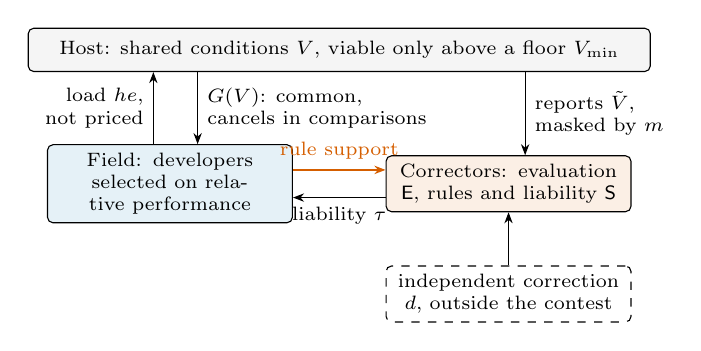
\begin{tikzpicture}[font=\scriptsize, box/.style={draw, rounded corners=2pt, align=center, inner sep=3pt}]
\node[box, minimum width=7.9cm, minimum height=0.55cm, fill=black!4] (host) at (0,2.25) {Host: shared conditions $V$, viable only above a floor $\Vmin$};
\node[box, fill=cD!10, text width=2.9cm] (field) at (-2.15,0.55) {Field: developers selected on relative performance};
\node[box, fill=cE!10, text width=2.9cm] (corr) at (2.15,0.55) {Correctors: evaluation $\dE$, rules and liability $\dS$};
\node[box, dashed, text width=2.9cm] (ind) at (2.15,-0.85) {independent correction $d$, outside the contest};
\draw[-{Stealth[length=4pt]}] ([xshift=-6pt]field.north) -- node[left, align=right]{load $he$,\\ not priced} ([xshift=-6pt]field.north |- host.south);
\draw[-{Stealth[length=4pt]}] ([xshift=10pt]field.north |- host.south) -- node[right, align=left]{$G(V)$: common,\\ cancels in comparisons} ([xshift=10pt]field.north);
\draw[-{Stealth[length=4pt]}] ([xshift=6pt]host.south -| corr.north) -- node[right, align=left]{reports $\tilde V$,\\ masked by $m$} ([xshift=6pt]corr.north);
\draw[-{Stealth[length=4pt]}, cE, thick] ([yshift=5pt]field.east) -- node[above]{rule support} ([yshift=5pt]corr.west);
\draw[-{Stealth[length=4pt]}] ([yshift=-5pt]corr.west) -- node[below]{liability $\tau$} ([yshift=-5pt]field.east);
\draw[-{Stealth[length=4pt]}] (ind.north) -- (corr.south);
\end{tikzpicture}
\caption{The model. Developers load a host they all depend on; selection compares them on relative performance, from which the host cancels (Section~\ref{sec:first}). Correctors can make costs return through liability, but success converts into rule support in the correctors (Section~\ref{sec:second}), and reports of the host are masked by captured evaluation (Section~\ref{sec:silent}).}
\label{fig:schematic}
\end{figure}

\paragraph{Host.} A condition $V\in[0,K]$ is shared by every participant: secure critical infrastructure, biosecurity, cyber stability, human control over AI systems, a reliable information environment. It regenerates logistically and is loaded by the field's activity $E$:
\begin{equation}\label{eq:V}
\dot V=V\big[\rho(1-V/K)-hE\big],\qquad \rho,h,K>0.
\end{equation}
For constant $E$ with $hE<\rho$, $V\to K(1-hE/\rho)$; for $hE\ge\rho$, $V\to0$. The host functions only above a floor $\Vmin\in(0,K)$, a normative line rather than an absorbing state. The host is the component of shared conditions whose costs do not return to their source through customers, reputation, courts or the source's own exposure; harms that do return are outside the model. Catastrophic tail risks fit the same structure, since a per-period probability of catastrophe borne by all is a term common to every payoff.

\begin{definition}[Viability]\label{def:viable}
A trajectory of the field is \emph{viable} if $V(t)\ge\Vmin$ for all $t\ge0$.
\end{definition}

Every participant persists only while the host does, so viability constrains every trajectory of the field rather than entering as one payoff among others: the field is a subsystem of a larger system \citep{aubin1991,rockstrom2009,wced1987}.

\paragraph{Field.} Carriers $k=1,\dots,n$ (developers or, more generally, reproducible ways of succeeding carried by organizations and their successors) hold shares $p_k$ of the field's activity: compute, capital, users, talent. Carrier $k$ runs a fraction $e_k\in[0,\bar e]$ of its activity in ways that load the host: deploying ahead of evaluation, omitting safeguards, entering contests in which capability converts directly into advantage. Each unit brings a private advantage $\nu>0$, so restraint costs $\nu$ per unit. The field's load is $E=\sum_kp_ke_k$, and carrier $k$'s absolute payoff is
\begin{equation}\label{eq:pi}
\pi_k=\phi_k+(\nu-\taueff)e_k+G(V),
\end{equation}
where $\phi_k$ collects everything else, $G$ is nondecreasing, and $\taueff\ge0$ is the effective liability imposed by correctors. With $\taueff=0$, $e_k=\bar e$ is the \emph{race strategy}.

\begin{definition}[Relative selection]\label{def:relsel}
A selection rule $\dot p=F(p,\pi)$ is \emph{relative} if $F(p,\pi+\xi\mathbf 1)=F(p,\pi)$ for every constant $\xi$, and \emph{payoff-monotone} if, for carriers $k,l$ present, $\dot p_k/p_k-\dot p_l/p_l$ has the sign of $\pi_k-\pi_l$.
\end{definition}

Replicator dynamics, pairwise imitation \citep{schlag1998}, logit choice on payoff differences and market-share competition driven by relative profitability \citep{alchian1950} are relative and payoff-monotone. Among a handful of frontier developers the operative reading is imitation of practices and the flow of capital, compute and talent to those ahead; between states only the strategic form of Section~\ref{sec:first} applies.

\paragraph{Correctors.} Correction makes costs return: an evaluator reports the host's condition, and rule-makers impose a liability $\tau$, in advance or when the reported condition $\tilde V$ falls to an alarm level $\Valarm\in(\Vmin,K)$. Correctors are not outside the field. Developers fund some evaluators, grant the access on which nearly all depend, author many benchmarks and standards contributions, and increasingly supply the models that judge. We represent this by a field of selection domains in which de facto power over rules is explicit \citep{acemoglu2008}. In domain $i$ (development $\dD$, evaluation $\dE$, rules and liability $\dS$, and others) a share $x_i$ of consequential decisions follows the dominant practice, and success converts into rule support $r_i$ that favors it:
\begin{align}
\dot x_i&=\kappa_ix_i(1-x_i)(a_ir_i-c_i),\label{eq:x}\\
\dot r_i&=\varepsilon_i\Big(\textstyle\sum_jb_{ij}x_j-d_ir_i\Big).\label{eq:r}
\end{align}
Under baseline rules ($r_i=0$) the practice carries a relative cost $c_i>0$ in domain $i$, which rule support offsets at rate $a_i$; $b_{ij}\ge0$ converts success in $j$ into rule support in $i$ (funding, personnel, authorship, data and infrastructure dependence, access terms); $d_i$ is the rate at which that support is corrected or decays. With $R_{ij}=a_ib_{ij}/(c_id_i)$ and inbound conversion $s_i(\cC)=\sum_{j\in\cC}R_{ij}$ from a set $\cC$: a domain whose full row sum $\sum_jR_{ij}$ is below one cannot be captured whatever happens elsewhere, and a seeded domain ($x_i>0$) with $s_i(\cC)>1$ is captured once $\cC$ is (Appendix~\ref{app:field}). In the corrector domains, $x_\dS$ is the share of rule-making that exempts or accommodates the practice, so $\taueff=\tau(1-x_\dS)$, and $x_\dE$ the share of evaluation conducted within the practice's lineage of funding, access, tooling, data and models. Capture here is structural: decisions follow the dominant practice through conversion channels, with or without intent \citep{kwak2014}. We do not claim that any present institution is captured; the model states when capture is selected. Independence means independence from the evaluated field, not any particular political form.

\paragraph{Maintained assumptions.} (A1) Exposure to the host is shared ($G$ common); Remark~\ref{rem:unequal} treats unequal exposure. (A2) Field size is fixed; with entry driven by absolute profit the host settles where rents dissipate \citep{gordon1954}, and C0 must then hold at that equilibrium. (A3) Conversion is monotone ($b_{ij}\ge0$), so countervailing pressure enters only through correction $d$ (Remark~\ref{rem:becker}). (A4) Costs of control are convex and fall with AI as a whole; a fixed part that AI does not lower caps the requirement (Proposition~\ref{prop:rate}v). (A5) Reports are averaged and non-strategic; a disjunctive alarm moves the problem from evaluation to rule-making (Section~\ref{sec:silent}). (A6) One practice and its alternative per domain, linear payoffs, uncalibrated parameters.

\section{First Order: Selection Does Not See the Host}\label{sec:first}

\begin{lemma}[Blindness]\label{lem:blind}
Under a relative rule, the trajectory of shares is unchanged by any term common to all payoffs, in particular by $G(V(t))$, whatever the path of $V$. Under a payoff-monotone rule, a common term never changes which of two carriers grows relative to the other.
\end{lemma}

The proof is one line; the content lies in (A1), that the host enters payoffs additively and identically.

\begin{proposition}[Selection drives the field toward the floor]\label{prop:first}
Let $\taueff=0$ and selection be payoff-monotone. (i) If $\phi_k=\phi_l$ and $e_k>e_l$, then $p_k/p_l$ increases while both are present, along every path of $V$, including paths below $\Vmin$. (ii) Under replicator dynamics, $\dot E=\nu\operatorname{Var}_p(e)+\operatorname{Cov}_p(e,\phi)$, so the race strategy spreads unless restraint is correlated with other sources of advantage, $\operatorname{Cov}_p(e,\phi)<-\nu\operatorname{Var}_p(e)$. (iii) If carriers differ only in load and a race-strategy carrier is present, $E(t)\to\bar e$ and $\limsup_tV(t)\le K(1-h\bar e/\rho)^+$; hence if
\begin{equation}\label{eq:C0}
h\bar e>\rho\,(1-\Vmin/K)\qquad\text{(C0)}
\end{equation}
$V$ eventually falls below the floor, however much any carrier values $V$.
\end{proposition}

What carriers value decides which strategies they try, not which ones grow. A developer that restrains itself because it values the shared condition is displaced unless restraint brings it other advantages, which for the host by definition it does not.

Selection is the limit of a contest in which only winning counts. Let $n\ge2$ symmetric developers with equal shares, $\taueff=0$ and the host at steady state choose $e_k$ to maximize $u_k=\pi_k+\lambda(\pi_k-\bar\pi)$, where $\bar\pi$ is the mean payoff and $\lambda\ge0$ is the \emph{weight on winning}: rank-based prizes, first-mover advantages, network effects, strategic rivalry in which falling behind is costly. Let $G(V)=\omega V$, $h\bar e<\rho$ and $\theta=\omega Kh/(\rho\nu)$, the value to the whole field of a unit of restraint relative to its private cost.

\begin{proposition}[The weight on winning]\label{prop:game}
(i) $G$ cancels from the relative term, and restraint is a dominant strategy if $1+\lambda(n-1)/n<\theta/n$, depletion if the inequality is reversed. (ii) If $\theta>1$, joint payoff is maximized by full restraint, while the equilibrium is full depletion whenever $\lambda>\bar\lambda=(\theta-n)/(n-1)$, at every $\lambda\ge0$ when $n>\theta$. (iii) In that equilibrium every developer's payoff is lower than under joint restraint, by $\nu\bar e(\theta-1)$. (iv) If $h\bar e>\rho(1-\Vmin/K)$, the equilibrium host lies below the floor although no developer chose it.
\end{proposition}

These comparative statics are those of \citet{armstrong2016} and of positional public-goods games; selection corresponds to $\lambda\to\infty$, the classical finding that selection maximizes relative payoff \citep{schaffer1988,schaffer1989}. Nothing here accuses anyone.

\begin{remark}[Thresholds and repetition]\label{rem:escape}
Strategic developers have two decentralized escapes. If crossing the floor costs each a common loss $L$, the relative term cancels $L$ but the absolute term does not, so a developer pivotal for crossing restrains when $L>(w-\theta/n)\nu\bar e$, with $w=1+\lambda(n-1)/n$, and the game becomes one of coordination at the threshold \citep{barrett2013}. In repeated play, joint restraint is sustained by reversion whenever the discount factor satisfies $\delta\ge(w-\theta/n)/(w-\theta/n+\theta-1)$; for $\theta=3$ and $n=4$ the cutoff is $0.11$ at $\lambda=0$, $0.47$ at $\lambda=2$ and $0.95$ at $\lambda=50$. Both escapes need observation: of where the floor lies, and of each developer's load. Uncertainty about the threshold turns coordination back into a dilemma \citep{barrettdannenberg2012}, and noisy monitoring makes reversion costly, with punishment triggered on the equilibrium path \citep{greenporter1984}. Section~\ref{sec:silent} shows that captured evaluation supplies both.
\end{remark}

\begin{remark}[The winner]\label{rem:winner}
A carrier that becomes the whole field faces $n=1$ and restrains whenever $\theta>1$ \citep{olson1993}. The trajectory of winning therefore fails through the race, not the winner: either the floor is crossed before the race ends, or rivalry continues after it (entry, rival states), so that relative selection persists. Hence our title.
\end{remark}

\paragraph{When the first order fails.} Lemma~\ref{lem:blind} needs (A1). If load returns to the carrier that caused it, $V$ enters payoff differences and selection can favor restraint, as in game--environment feedback \citep{weitz2016,tilman2020}. Making consequences return to their source is the corrector's task. The question is whether correctors survive the selection they correct.

\section{Second Order: The Corrector Is Selected}\label{sec:second}

\paragraph{Control over correctors.} Rule support can be incidental, as when benchmarks are built from deployed systems, or cultivated. Carriers differ in \emph{conversion capacity} $q\ge0$: investment in drafting standards, building evaluation tooling, authoring benchmarks, funding evaluators and securing integrations. A unit of capacity converts the carrier's own success into rule support at rate $\hat b_{ij}$, and a fraction $\chi\in[0,1]$ of that support, the \emph{appropriability}, is keyed to the carrier (standards referencing its interfaces, evaluations run on its tooling). A carrier with share $p$ of decisions distributed by a profile $\bar y$ ($y=p\bar y$) and capacity cost $C(q)=fq+\gamma q^{1+\eta}/(1+\eta)$, $\eta>0$, earns, relative to an otherwise identical carrier with $q=0$ and averaged over a selection horizon,
\begin{equation}\label{eq:W}
W(q)=\chi q\,y^\top My-C(q),\qquad M_{ij}=c_iL_i\hat R_{ij},
\end{equation}
where $\hat R_{ij}=a_i\hat b_{ij}/(c_id_i)$ and $L_i\in[0,1)$ is the share of the steady-state return realized within the horizon; $L_i$ rises with $d_i$ but $L_i/d_i$ falls.

\begin{proposition}[Control is selected in the largest carriers]\label{prop:control}
(i) The local selection gradient is $W'(q)=\chi p^2\,\bar y^\top M\bar y-C'(q)$; under faithful transmission with variation, mean capacity rises when $W$ is increasing on the trait support. (ii) Capacity pays only above the size threshold $p^\ast=\sqrt{f/(\chi\,\bar y^\top M\bar y)}$: a carrier with smaller share that carries capacity is selected against. (iii) The return rises with $\chi$ and every $\hat b_{ij}$, falls with every correction rate $d_i$, and vanishes if $\chi=0$. (iv) With share $p$ in each domain of a set $\cS$, $\hat R$ equal to $\hat\eta$ on and $\hat\varphi$ off the diagonal and $c_iL_i=cL$, the return is $\chi cL\,p^2|\cS|(\hat\eta+(|\cS|-1)\hat\varphi)$, superlinear in $|\cS|$ at fixed $p$ when $\hat\varphi>0$; at fixed total size it rises with scope only if $\hat\varphi>\hat\eta$.
\end{proposition}

Control over correctors amplifies dominance rather than creating it: it is selected in carriers that are already large, in proportion to the square of their share. The condition has the form of Hamilton's rule with appropriability in the role of relatedness \citep{hamilton1964,price1970}; it parallels fixed-cost participation in lobbying \citep{bombardini2008} and appropriability in niche construction \citep{krakauer2009,lehmann2008,gerlee2015}.

\paragraph{Correction of correctors.} Let carriers also differ in an investment $u\ge0$, at private cost $C_u(u)$ with $C_u'>0$, that raises the correction rate $d$ of rule support in the corrector domains for everyone.

\begin{proposition}[Correction is not supplied from inside]\label{prop:correction}
(i) Among otherwise identical carriers of the same practice, those investing more in correction are selected against under any payoff-monotone rule, whatever the effect of correction on the field. (ii) Holding the host fixed, correction lowers the payoff of a carrier that holds rule support, so incumbents oppose it. (iii) In absolute terms a challenger invests only if its own share of the benefit exceeds $C_u'(0)$, so dispersed challengers free-ride. (iv) Correction whose benefit is keyed to the corrector, because it installs the corrector's own rule support, is control in the sense of Proposition~\ref{prop:control}, selected above the size threshold; it replaces one captured configuration with another. (v) If $\theta>1$ and correction is what makes liability effective, an incumbent can gain from correction applied to all carriers; it opposes correction applied to itself alone.
\end{proposition}

Correction can rise transiently by riding on the success of the practice it favors, the between-group term of the Price equation; within any practice part (i) applies, and once that practice dominates it is the incumbent. Independent correction, which restores baseline rules and is keyed to no one, is a second-order public good \citep{oliver1980,yamagishi1986,heckathorn1989}. It is sustained by reputation or by competition among institutions only when contributions and outcomes are observed \citep{panchanathan2004,gurerk2006,sigmund2010}.

\paragraph{How much independent correction, and how fast.} Let a set $\cC\not\ni\dE$ be captured by a dominant carrier that holds it ($y_j=1$ on $\cC$), let all conversion into $\dE$ originate in $\cC$, so that $s_\dE(\cC)$ is $\dE$'s full row sum, and let cultivated conversion enter only the corrector domains, where independent correction acts at a uniform rate $d$. Take $f=0$ and capacity at its selected level $q^\ast(d,\gamma)$. In the long-horizon limit ($L_i\to1$), $q^\ast=(\chi\hat Y/(\gamma d))^{1/\eta}$ with $\hat Y=\sum_{ij}y_ia_i\hat b_{ij}y_j$, and
\begin{equation}\label{eq:sE}
s_\dE=\frac{A+a_\dE\hat B\,q^\ast}{c_\dE d},\quad A=a_\dE\!\sum_{j\in\cC}b^0_{\dE j},\ \hat B=\sum_{j\in\cC}\hat b_{\dE j}.
\end{equation}

\begin{proposition}[Required independent correction, and its rate]\label{prop:rate}
(i) $s_\dE$ decreases in $d$, and evaluation is certified uncaptured iff $d>d^\ast(\gamma)$, the root of $s_\dE=1$; for $\eta=1$, $d^\ast=\big(A+\sqrt{A^2+4c_\dE Z}\big)/(2c_\dE)$ with $Z=a_\dE\hat B\chi\hat Y/\gamma$. (ii) $d^\ast\ge A/c_\dE$, the requirement without second-order selection, with equality iff $\chi\hat B\hat Y=0$; $d^\ast$ rises with appropriability, with the dominant carrier's size and, at fixed share per domain, its scope, and as $\gamma$ falls. (iii) Let AI lower the cost of control as $\gamma(t)=\gamma_0e^{-gt}$ and independent correction grow as $d(t)=d_0e^{\alpha t}$. If $\alpha\ge g/(1+\eta)$, the certificate holds for all $t$ iff $d_0>d^\ast(\gamma_0)$. If $\alpha<g/(1+\eta)$, it fails for all $t$ beyond a finite time, after which a seeded evaluation domain is captured. If the selection horizon is short relative to the life of rule support, the threshold is $g/\eta$ instead. (iv) If AI lowers the unit cost of independent correction at rate $g_c$ and its budget grows at rate $b$, then $\alpha=b+g_c$, and capture requires $g>(1+\eta)(b+g_c)$. (v) With a fixed part $f>0$ of the cost of control that falls at rate $g_f$, the required rate is $\min\{g_f,g/(1+\eta)\}$; if $f$ does not fall, the requirement levels off at $\max\{A/c_\dE,\chi\hat Y/f\}$. The same holds for $\dS$.
\end{proposition}

Independent correction does double duty: it shortens the life of rule support and shrinks the capacity that selection cultivates, which is why under quadratic cost ($\eta=1$) and long horizons it needs to grow only half as fast as the cost of control falls. Splitting a dominant carrier into $k$ equal parts divides cultivated conversion by $k^2$: each part's selected capacity falls with the square of its share, and each converts only its own success.

\paragraph{What AI changes.} AI lowers the cost of what control consists of: models already write evaluation datasets \citep{perez2023}, and machine-written public comments and letters to legislators pass as human \citep{weiss2019,kreps2024}. But writing evaluations is also what independent correctors do. By Proposition~\ref{prop:rate}(iv), whether AI favors capture depends on two rates, how fast it cheapens control and how fast it cheapens independent correction; capture is favored only if the first exceeds the second, plus budget growth, by the factor $1+\eta$. Aligning each system to its operator does not change this, since a faithful assistant lowers its principal's cost of control as much as any capability does; what changes it is whether independent correctors adopt AI as fast as the field does. General-purpose providers are present in many domains, which raises the return to control (Proposition~\ref{prop:control}iv), and model judges put the evaluated lineage in the selector's seat (Section~\ref{sec:silent}).

\begin{remark}[Countervailing pressure]\label{rem:becker}
Following \citet{becker1983}, let those harmed mobilize in proportion to the harm they perceive, so that independent correction responds to reports, $d=d_0+\varkappa(K-\tilde V)$. With accurate reports this feedback stabilizes the uncaptured state; with masking $m$ it is disabled exactly when needed, since $K-\tilde V=(1-m)(K-V)$.
\end{remark}

\section{Observation: Silent Descent}\label{sec:silent}

Reports average over evaluators. A fraction $x_\dE$ shares the evaluated lineage and reports the condition a fraction $\beta_{\mathrm{in}}$ of the way toward full health; the rest, formed on shared material, are biased by $\beta_{\mathrm{out}}$, with $0\le\beta_{\mathrm{out}}\le\beta_{\mathrm{in}}<1$:
\begin{equation}\label{eq:mask}
\tilde V=V+m(K-V),\qquad m=x_\dE\beta_{\mathrm{in}}+(1-x_\dE)\beta_{\mathrm{out}}.
\end{equation}
For frontier evaluation, $\beta_{\mathrm{in}}$ stands for short access windows set by the evaluated developer, under-elicitation, evaluation awareness and sandbagging \citep{metr2025o3,vanderweij2024,needham2025,bengio2026report}, and for lineage preference of model judges \citep{panickssery2024}; $\beta_{\mathrm{out}}$ for shared training data, homogenized judges and lost data access \citep{kleinberg2021,bommasani2022}. Masking is a property of the corrector's payoff as well as its lineage: an evaluator that bears the loss of a false report, such as an insurer or a liable gatekeeper, has $\beta\le0$ \citep{kraakman1986,benshahar2012}. The alarm fires at the first $t$ with $\tilde V(t)\le\Valarm$. Let $\mfl=(\Valarm-\Vmin)/(K-\Vmin)$.

\begin{proposition}[Detection]\label{prop:detect}
(i) The alarm fires only once $V\le(\Valarm-mK)/(1-m)$, a level that falls as $m$ rises. (ii) \emph{Silent crossing.} If $m(t)>\mfl$ whenever $\Vmin\le V(t)\le\Valarm$, the alarm does not fire before $V$ falls below the floor. (iii) \emph{Permanent silence of moderate harm.} If $V$ decreases to $V^\ast\in(0,\Valarm)$ and $m(t)\ge\bar m>(\Valarm-V^\ast)/(K-V^\ast)$ for all $t$, the alarm never fires; the masking required vanishes as $V^\ast\uparrow\Valarm$. (iv) If $V\to0$ and eventually $m\le m_1<\Valarm/K$, the alarm fires. (v) If $V$ reaches $\Valarm$ at $t_A$ and then declines as $\dot V=-\ell V$ with $m<\Valarm/K$ constant, the alarm is delayed by $\ell^{-1}\ln\big[(1-m)\Valarm/(\Valarm-mK)\big]$, which diverges as $m\uparrow\Valarm/K$.
\end{proposition}

Part (iii) concerns harm that stays above the floor, so it bears on what is known, not on viability. Diverse panels reduce some error: with equicorrelated errors of variance $\sigma^2$ and correlation $r$, averaging $n$ evaluators leaves $\sigma^2[r+(1-r)/n]$; but family diversity alone does not bound shared systematic masking $\beta_{\mathrm{out}}$, and a report of unknown composition cannot be recalibrated without an independent channel (Remark~\ref{rem:indist}). If the alarm fires on any credible report instead of the average, silent crossing requires $\beta_{\mathrm{out}}>\mfl$, and the outcome turns on whether a captured rule-making domain ($x_\dS$) acts on the dissent. Detection is not correction: deciding takes $T_d$ and reversing takes $T_r$, both before the floor.

\paragraph{Masking defeats the decentralized escapes.} Each escape from the first-order dilemma runs on accurate observation of the host or of loads: coordination at a known threshold and reversion in repeated play (Remark~\ref{rem:escape}), reputation that sustains sanctioning \citep{panchanathan2004}, countervailing pressure (Remark~\ref{rem:becker}), and insurers' pricing. Captured evaluation degrades all of them at once. The problem is not only that selection cannot see the host; captured evaluation keeps everyone from seeing it, including strategic players who could otherwise cooperate on their own.

\begin{figure}[t]
\centering
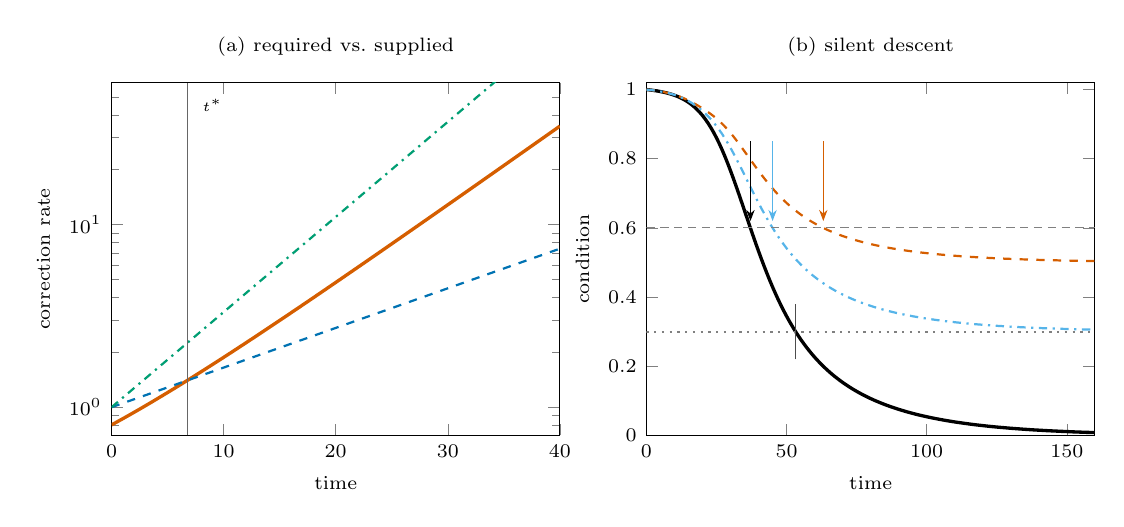
\begin{tikzpicture}
\begin{groupplot}[group style={group size=2 by 1, horizontal sep=1.1cm}, width=0.6\columnwidth, height=0.5\columnwidth,
  tick label style={font=\scriptsize}, label style={font=\scriptsize}, title style={font=\scriptsize}]
\nextgroupplot[ymode=log, xmin=0, xmax=40, ymin=0.7, ymax=60, xlabel={time}, ylabel={correction rate}, title={(a) required vs.\ supplied}]
\addplot[cE, very thick] coordinates {(0.00,0.8000) (0.50,0.8316) (1.00,0.8649) (1.50,0.9000) (2.00,0.9369) (2.50,0.9758) (3.00,1.0168) (3.50,1.0599) (4.00,1.1054) (4.50,1.1532) (5.00,1.2035) (5.50,1.2564) (6.00,1.3121) (6.50,1.3707) (7.00,1.4324) (7.50,1.4973) (8.00,1.5655) (8.50,1.6373) (9.00,1.7128) (9.50,1.7922) (10.00,1.8757) (10.50,1.9636) (11.00,2.0559) (11.50,2.1530) (12.00,2.2552) (12.50,2.3626) (13.00,2.4755) (13.50,2.5943) (14.00,2.7191) (14.50,2.8504) (15.00,2.9884) (15.50,3.1336) (16.00,3.2862) (16.50,3.4466) (17.00,3.6153) (17.50,3.7926) (18.00,3.9791) (18.50,4.1751) (19.00,4.3812) (19.50,4.5979) (20.00,4.8257) (20.50,5.0651) (21.00,5.3169) (21.50,5.5816) (22.00,5.8599) (22.50,6.1524) (23.00,6.4600) (23.50,6.7834) (24.00,7.1233) (24.50,7.4806) (25.00,7.8563) (25.50,8.2513) (26.00,8.6665) (26.50,9.1031) (27.00,9.5620) (27.50,10.0444) (28.00,10.5516) (28.50,11.0848) (29.00,11.6453) (29.50,12.2346) (30.00,12.8541) (30.50,13.5054) (31.00,14.1900) (31.50,14.9098) (32.00,15.6665) (32.50,16.4619) (33.00,17.2982) (33.50,18.1773) (34.00,19.1016) (34.50,20.0732) (35.00,21.0946) (35.50,22.1684) (36.00,23.2972) (36.50,24.4840) (37.00,25.7316) (37.50,27.0431) (38.00,28.4219) (38.50,29.8714) (39.00,31.3952) (39.50,32.9972) (40.00,34.6812)};\label{pl:dstar}
\addplot[cD, thick, dashed] coordinates {(0.00,1.0000) (0.50,1.0253) (1.00,1.0513) (1.50,1.0779) (2.00,1.1052) (2.50,1.1331) (3.00,1.1618) (3.50,1.1912) (4.00,1.2214) (4.50,1.2523) (5.00,1.2840) (5.50,1.3165) (6.00,1.3499) (6.50,1.3840) (7.00,1.4191) (7.50,1.4550) (8.00,1.4918) (8.50,1.5296) (9.00,1.5683) (9.50,1.6080) (10.00,1.6487) (10.50,1.6905) (11.00,1.7333) (11.50,1.7771) (12.00,1.8221) (12.50,1.8682) (13.00,1.9155) (13.50,1.9640) (14.00,2.0138) (14.50,2.0647) (15.00,2.1170) (15.50,2.1706) (16.00,2.2255) (16.50,2.2819) (17.00,2.3396) (17.50,2.3989) (18.00,2.4596) (18.50,2.5219) (19.00,2.5857) (19.50,2.6512) (20.00,2.7183) (20.50,2.7871) (21.00,2.8577) (21.50,2.9300) (22.00,3.0042) (22.50,3.0802) (23.00,3.1582) (23.50,3.2381) (24.00,3.3201) (24.50,3.4042) (25.00,3.4903) (25.50,3.5787) (26.00,3.6693) (26.50,3.7622) (27.00,3.8574) (27.50,3.9551) (28.00,4.0552) (28.50,4.1579) (29.00,4.2631) (29.50,4.3710) (30.00,4.4817) (30.50,4.5951) (31.00,4.7115) (31.50,4.8307) (32.00,4.9530) (32.50,5.0784) (33.00,5.2070) (33.50,5.3388) (34.00,5.4739) (34.50,5.6125) (35.00,5.7546) (35.50,5.9003) (36.00,6.0496) (36.50,6.2028) (37.00,6.3598) (37.50,6.5208) (38.00,6.6859) (38.50,6.8551) (39.00,7.0287) (39.50,7.2066) (40.00,7.3891)};\label{pl:dlow}
\addplot[cS, thick, dashdotted] coordinates {(0.00,1.0000) (0.50,1.0618) (1.00,1.1275) (1.50,1.1972) (2.00,1.2712) (2.50,1.3499) (3.00,1.4333) (3.50,1.5220) (4.00,1.6161) (4.50,1.7160) (5.00,1.8221) (5.50,1.9348) (6.00,2.0544) (6.50,2.1815) (7.00,2.3164) (7.50,2.4596) (8.00,2.6117) (8.50,2.7732) (9.00,2.9447) (9.50,3.1268) (10.00,3.3201) (10.50,3.5254) (11.00,3.7434) (11.50,3.9749) (12.00,4.2207) (12.50,4.4817) (13.00,4.7588) (13.50,5.0531) (14.00,5.3656) (14.50,5.6973) (15.00,6.0496) (15.50,6.4237) (16.00,6.8210) (16.50,7.2427) (17.00,7.6906) (17.50,8.1662) (18.00,8.6711) (18.50,9.2073) (19.00,9.7767) (19.50,10.3812) (20.00,11.0232) (20.50,11.7048) (21.00,12.4286) (21.50,13.1971) (22.00,14.0132) (22.50,14.8797) (23.00,15.7998) (23.50,16.7769) (24.00,17.8143) (24.50,18.9158) (25.00,20.0855) (25.50,21.3276) (26.00,22.6464) (26.50,24.0468) (27.00,25.5337) (27.50,27.1126) (28.00,28.7892) (28.50,30.5694) (29.00,32.4597) (29.50,34.4669) (30.00,36.5982) (30.50,38.8613) (31.00,41.2644) (31.50,43.8160) (32.00,46.5255) (32.50,49.4024) (33.00,52.4573) (33.50,55.7011) (34.00,59.1455) (34.50,62.8028) (35.00,66.6863) (35.50,70.8100) (36.00,75.1886) (36.50,79.8380) (37.00,84.7749) (37.50,90.0171) (38.00,95.5835) (38.50,101.4940) (39.00,107.7701) (39.50,114.4342) (40.00,121.5104)};\label{pl:dhigh}
\draw[black!60] (axis cs:6.76,0.7) -- (axis cs:6.76,60);
\node[font=\tiny, anchor=north west] at (axis cs:7.26,55) {$t^\ast$};
\nextgroupplot[xmin=0, xmax=160, ymin=0, ymax=1.02, xlabel={time}, ylabel={condition}, title={(b) silent descent}]
\addplot[black, very thick] coordinates {(0.00,1.0000) (1.00,0.9991) (2.00,0.9981) (3.00,0.9969) (4.00,0.9956) (5.00,0.9942) (6.00,0.9925) (7.00,0.9907) (8.00,0.9886) (9.00,0.9862) (10.00,0.9834) (11.00,0.9803) (12.00,0.9768) (13.00,0.9727) (14.00,0.9681) (15.00,0.9629) (16.00,0.9570) (17.00,0.9503) (18.00,0.9428) (19.00,0.9343) (20.00,0.9248) (21.00,0.9142) (22.00,0.9025) (23.00,0.8896) (24.00,0.8755) (25.00,0.8600) (26.00,0.8434) (27.00,0.8255) (28.00,0.8064) (29.00,0.7862) (30.00,0.7650) (31.00,0.7430) (32.00,0.7203) (33.00,0.6970) (34.00,0.6734) (35.00,0.6495) (36.00,0.6256) (37.00,0.6018) (38.00,0.5783) (39.00,0.5551) (40.00,0.5325) (41.00,0.5104) (42.00,0.4890) (43.00,0.4683) (44.00,0.4483) (45.00,0.4291) (46.00,0.4107) (47.00,0.3930) (48.00,0.3762) (49.00,0.3601) (50.00,0.3447) (51.00,0.3301) (52.00,0.3162) (53.00,0.3029) (54.00,0.2903) (55.00,0.2783) (56.00,0.2669) (57.00,0.2560) (58.00,0.2457) (59.00,0.2358) (60.00,0.2264) (61.00,0.2175) (62.00,0.2090) (63.00,0.2008) (64.00,0.1931) (65.00,0.1857) (66.00,0.1786) (67.00,0.1719) (68.00,0.1655) (69.00,0.1593) (70.00,0.1534) (71.00,0.1478) (72.00,0.1424) (73.00,0.1373) (74.00,0.1323) (75.00,0.1276) (76.00,0.1231) (77.00,0.1187) (78.00,0.1145) (79.00,0.1105) (80.00,0.1067) (81.00,0.1030) (82.00,0.0995) (83.00,0.0961) (84.00,0.0928) (85.00,0.0896) (86.00,0.0866) (87.00,0.0837) (88.00,0.0809) (89.00,0.0782) (90.00,0.0756) (91.00,0.0731) (92.00,0.0707) (93.00,0.0683) (94.00,0.0661) (95.00,0.0639) (96.00,0.0618) (97.00,0.0598) (98.00,0.0579) (99.00,0.0560) (100.00,0.0542) (101.00,0.0525) (102.00,0.0508) (103.00,0.0492) (104.00,0.0476) (105.00,0.0461) (106.00,0.0446) (107.00,0.0432) (108.00,0.0418) (109.00,0.0405) (110.00,0.0392) (111.00,0.0380) (112.00,0.0368) (113.00,0.0357) (114.00,0.0346) (115.00,0.0335) (116.00,0.0324) (117.00,0.0314) (118.00,0.0304) (119.00,0.0295) (120.00,0.0286) (121.00,0.0277) (122.00,0.0268) (123.00,0.0260) (124.00,0.0252) (125.00,0.0244) (126.00,0.0237) (127.00,0.0230) (128.00,0.0223) (129.00,0.0216) (130.00,0.0209) (131.00,0.0203) (132.00,0.0197) (133.00,0.0191) (134.00,0.0185) (135.00,0.0179) (136.00,0.0174) (137.00,0.0168) (138.00,0.0163) (139.00,0.0158) (140.00,0.0154) (141.00,0.0149) (142.00,0.0144) (143.00,0.0140) (144.00,0.0136) (145.00,0.0132) (146.00,0.0128) (147.00,0.0124) (148.00,0.0120) (149.00,0.0117) (150.00,0.0113) (151.00,0.0110) (152.00,0.0106) (153.00,0.0103) (154.00,0.0100) (155.00,0.0097) (156.00,0.0094) (157.00,0.0091) (158.00,0.0089) (159.00,0.0086) (160.00,0.0083)};\label{pl:Vtrue}
\addplot[cE, thick, dashed] coordinates {(0.00,1.0000) (1.00,0.9991) (2.00,0.9982) (3.00,0.9971) (4.00,0.9959) (5.00,0.9945) (6.00,0.9930) (7.00,0.9913) (8.00,0.9894) (9.00,0.9872) (10.00,0.9848) (11.00,0.9822) (12.00,0.9792) (13.00,0.9759) (14.00,0.9724) (15.00,0.9685) (16.00,0.9644) (17.00,0.9600) (18.00,0.9554) (19.00,0.9505) (20.00,0.9455) (21.00,0.9402) (22.00,0.9347) (23.00,0.9289) (24.00,0.9227) (25.00,0.9160) (26.00,0.9088) (27.00,0.9011) (28.00,0.8928) (29.00,0.8839) (30.00,0.8745) (31.00,0.8646) (32.00,0.8542) (33.00,0.8434) (34.00,0.8324) (35.00,0.8211) (36.00,0.8098) (37.00,0.7984) (38.00,0.7871) (39.00,0.7759) (40.00,0.7648) (41.00,0.7541) (42.00,0.7436) (43.00,0.7334) (44.00,0.7235) (45.00,0.7141) (46.00,0.7049) (47.00,0.6962) (48.00,0.6878) (49.00,0.6798) (50.00,0.6722) (51.00,0.6649) (52.00,0.6580) (53.00,0.6514) (54.00,0.6451) (55.00,0.6391) (56.00,0.6334) (57.00,0.6280) (58.00,0.6228) (59.00,0.6179) (60.00,0.6132) (61.00,0.6087) (62.00,0.6045) (63.00,0.6004) (64.00,0.5965) (65.00,0.5928) (66.00,0.5893) (67.00,0.5859) (68.00,0.5827) (69.00,0.5797) (70.00,0.5767) (71.00,0.5739) (72.00,0.5712) (73.00,0.5686) (74.00,0.5662) (75.00,0.5638) (76.00,0.5615) (77.00,0.5594) (78.00,0.5573) (79.00,0.5553) (80.00,0.5534) (81.00,0.5515) (82.00,0.5497) (83.00,0.5480) (84.00,0.5464) (85.00,0.5448) (86.00,0.5433) (87.00,0.5418) (88.00,0.5404) (89.00,0.5391) (90.00,0.5378) (91.00,0.5365) (92.00,0.5353) (93.00,0.5342) (94.00,0.5330) (95.00,0.5320) (96.00,0.5309) (97.00,0.5299) (98.00,0.5289) (99.00,0.5280) (100.00,0.5271) (101.00,0.5262) (102.00,0.5254) (103.00,0.5246) (104.00,0.5238) (105.00,0.5230) (106.00,0.5223) (107.00,0.5216) (108.00,0.5209) (109.00,0.5203) (110.00,0.5196) (111.00,0.5190) (112.00,0.5184) (113.00,0.5178) (114.00,0.5173) (115.00,0.5167) (116.00,0.5162) (117.00,0.5157) (118.00,0.5152) (119.00,0.5148) (120.00,0.5143) (121.00,0.5139) (122.00,0.5134) (123.00,0.5130) (124.00,0.5126) (125.00,0.5122) (126.00,0.5118) (127.00,0.5115) (128.00,0.5111) (129.00,0.5108) (130.00,0.5105) (131.00,0.5101) (132.00,0.5098) (133.00,0.5095) (134.00,0.5092) (135.00,0.5090) (136.00,0.5087) (137.00,0.5084) (138.00,0.5082) (139.00,0.5079) (140.00,0.5077) (141.00,0.5074) (142.00,0.5072) (143.00,0.5070) (144.00,0.5068) (145.00,0.5066) (146.00,0.5064) (147.00,0.5062) (148.00,0.5060) (149.00,0.5058) (150.00,0.5057) (151.00,0.5055) (152.00,0.5053) (153.00,0.5052) (154.00,0.5050) (155.00,0.5049) (156.00,0.5047) (157.00,0.5046) (158.00,0.5044) (159.00,0.5043) (160.00,0.5042)};\label{pl:V5}
\addplot[cP, thick, dashdotted] coordinates {(0.00,1.0000) (1.00,0.9991) (2.00,0.9982) (3.00,0.9971) (4.00,0.9959) (5.00,0.9945) (6.00,0.9930) (7.00,0.9912) (8.00,0.9893) (9.00,0.9871) (10.00,0.9846) (11.00,0.9818) (12.00,0.9786) (13.00,0.9751) (14.00,0.9712) (15.00,0.9668) (16.00,0.9620) (17.00,0.9568) (18.00,0.9510) (19.00,0.9448) (20.00,0.9380) (21.00,0.9306) (22.00,0.9226) (23.00,0.9139) (24.00,0.9044) (25.00,0.8942) (26.00,0.8832) (27.00,0.8714) (28.00,0.8587) (29.00,0.8452) (30.00,0.8311) (31.00,0.8163) (32.00,0.8009) (33.00,0.7851) (34.00,0.7690) (35.00,0.7527) (36.00,0.7363) (37.00,0.7199) (38.00,0.7036) (39.00,0.6876) (40.00,0.6720) (41.00,0.6566) (42.00,0.6418) (43.00,0.6274) (44.00,0.6135) (45.00,0.6001) (46.00,0.5873) (47.00,0.5750) (48.00,0.5632) (49.00,0.5520) (50.00,0.5412) (51.00,0.5310) (52.00,0.5213) (53.00,0.5120) (54.00,0.5032) (55.00,0.4948) (56.00,0.4868) (57.00,0.4792) (58.00,0.4719) (59.00,0.4650) (60.00,0.4585) (61.00,0.4522) (62.00,0.4463) (63.00,0.4406) (64.00,0.4352) (65.00,0.4300) (66.00,0.4250) (67.00,0.4203) (68.00,0.4158) (69.00,0.4115) (70.00,0.4074) (71.00,0.4035) (72.00,0.3997) (73.00,0.3961) (74.00,0.3926) (75.00,0.3893) (76.00,0.3861) (77.00,0.3831) (78.00,0.3802) (79.00,0.3774) (80.00,0.3747) (81.00,0.3721) (82.00,0.3696) (83.00,0.3672) (84.00,0.3649) (85.00,0.3627) (86.00,0.3606) (87.00,0.3586) (88.00,0.3566) (89.00,0.3547) (90.00,0.3529) (91.00,0.3511) (92.00,0.3495) (93.00,0.3478) (94.00,0.3463) (95.00,0.3447) (96.00,0.3433) (97.00,0.3419) (98.00,0.3405) (99.00,0.3392) (100.00,0.3380) (101.00,0.3367) (102.00,0.3356) (103.00,0.3344) (104.00,0.3333) (105.00,0.3323) (106.00,0.3312) (107.00,0.3302) (108.00,0.3293) (109.00,0.3284) (110.00,0.3275) (111.00,0.3266) (112.00,0.3258) (113.00,0.3250) (114.00,0.3242) (115.00,0.3234) (116.00,0.3227) (117.00,0.3220) (118.00,0.3213) (119.00,0.3207) (120.00,0.3200) (121.00,0.3194) (122.00,0.3188) (123.00,0.3182) (124.00,0.3177) (125.00,0.3171) (126.00,0.3166) (127.00,0.3161) (128.00,0.3156) (129.00,0.3151) (130.00,0.3146) (131.00,0.3142) (132.00,0.3138) (133.00,0.3133) (134.00,0.3129) (135.00,0.3125) (136.00,0.3122) (137.00,0.3118) (138.00,0.3114) (139.00,0.3111) (140.00,0.3107) (141.00,0.3104) (142.00,0.3101) (143.00,0.3098) (144.00,0.3095) (145.00,0.3092) (146.00,0.3089) (147.00,0.3087) (148.00,0.3084) (149.00,0.3082) (150.00,0.3079) (151.00,0.3077) (152.00,0.3074) (153.00,0.3072) (154.00,0.3070) (155.00,0.3068) (156.00,0.3066) (157.00,0.3064) (158.00,0.3062) (159.00,0.3060) (160.00,0.3058)};\label{pl:V3}
\draw[black!50, densely dashed] (axis cs:0,0.6) -- (axis cs:160,0.6);
\draw[black!50, dotted, thick] (axis cs:0,0.3) -- (axis cs:160,0.3);
\draw[-{Stealth[length=4pt]}, black] (axis cs:37.1,0.85) -- (axis cs:37.1,0.62);
\draw[-{Stealth[length=4pt]}, cP] (axis cs:45.0,0.85) -- (axis cs:45.0,0.62);
\draw[-{Stealth[length=4pt]}, cE] (axis cs:63.1,0.85) -- (axis cs:63.1,0.62);
\draw[black!70] (axis cs:53.2,0.22) -- (axis cs:53.2,0.38);
\end{groupplot}
\end{tikzpicture}

\caption{(a) Required independent correction $d^\ast(t)$ (\ref{pl:dstar}) as AI lowers the cost of control ($g=0.2$; quadratic cost, long horizon), against correction growing at $\alpha=0.05<g/2$ (\ref{pl:dlow}), overtaken at $t_c\approx6.8$ (bound $t^\ast\approx9.2$), and at $\alpha=0.12>g/2$ (\ref{pl:dhigh}), which is not. (b) The host $V$ (\ref{pl:Vtrue}) under a spreading race strategy, and reports when evaluation is captured before the harm appears, with $\beta_{\mathrm{in}}=0.5>\mfl$ (\ref{pl:V5}) and $0.3$ (\ref{pl:V3}). Arrows: alarms with independent evaluation ($t\approx37$), at $\beta_{\mathrm{in}}=0.3$ ($t\approx45$) and at $0.5$ ($t\approx63$), after the floor (dotted) is crossed at $t\approx53$ (tick). Appendix~\ref{app:numerics}.}
\label{fig:rate}
\end{figure}

Figure~\ref{fig:rate}b shows the regimes. Independent evaluation raises the alarm sixteen time units before the floor; masking below $\mfl$ halves that window; masking above it raises the alarm ten time units after the floor. When evaluation is captured only after the harm appears, the alarm fires almost on time: the order of capture and evidence decides the outcome.

\section{Why the Race Fails}\label{sec:fail}

\begin{theorem}[No viable race]\label{thm:fail}
Assume (C0) Eq.~(\ref{eq:C0}); (C1) replicator selection among carriers that differ only in load, a race-strategy carrier present, and $\taueff<\nu$ unless an alarm fires; (C2) appropriable control, $\chi>0$, with the whole cost of control falling with AI; (C3) the hypotheses of Proposition~\ref{prop:rate}(iii) with $\alpha<g/(1+\eta)$, $\cC$ captured and $\dE$ seeded; (C4) $0\le\beta_{\mathrm{out}}<\mfl<\beta_{\mathrm{in}}<1$; and (C6) capture before evidence: $x_\dE(t)>(\mfl-\beta_{\mathrm{out}})/(\beta_{\mathrm{in}}-\beta_{\mathrm{out}})$ whenever $\Vmin\le V(t)\le\Valarm$. Then the host crosses its floor before any alarm. If instead $\beta_{\mathrm{in}}\le\mfl$, the alarm is delayed (Proposition~\ref{prop:detect}i), and the floor is crossed unless $T_d+T_r$ fits the remaining window and a liability enacted against a captured $\dS$ is not re-absorbed (Proposition~\ref{prop:reform}iii).
\end{theorem}

Condition C6 can be checked from two clocks. The host cannot reach the alarm level before $T_A=(\rho-h\bar e)^{-1}\ln[(1-V^\ast/V_0)/(1-V^\ast/\Valarm)]$ with $V^\ast=K(1-h\bar e/\rho)$ (when $h\bar e<\rho$), since $E\le\bar e$; the certificate of evaluation fails within the bound $t^\ast$ of Proposition~\ref{prop:rate}, which shrinks as AI cheapens control faster. Acceleration can bring both forward, so C6 is a condition to be checked, not a consequence.

When $G(V)=\omega V$ and $\omega K\min\{1,h\bar e/\rho\}>\nu\bar e$ ($\theta>1$ when $h\bar e\le\rho$), every carrier's limiting payoff (\ref{eq:pi}), with $\phi_k$ the same in both outcomes, is lower in the race than under joint restraint (C5 in Table~\ref{tab:evidence}). This comparison excludes the rents of control over correctors, which accrue to the largest carriers.

\begin{remark}[Unequal exposure]\label{rem:unequal}
If a carrier's exposure to the host falls with its share, because it can buy private substitutes for shared conditions or because a captured corrector favors it, the host no longer cancels from comparisons involving it, and selection favors insulation as well as load. Either exposure is shared, and no carrier's trajectory is viable once the host crosses its floor; or it is not, and a carrier may remain viable while the host does not. That is a concentration of power over everyone who depends on the host, which the contestability premise of Section~\ref{sec:conclusion} excludes. Neither branch yields a trajectory acceptable to those who depend on the host.
\end{remark}

\begin{table*}[t]
\centering
\small
\setlength{\tabcolsep}{3.5pt}
\begin{tabular}{@{}>{\raggedright\arraybackslash}p{3.2cm}>{\raggedright\arraybackslash}p{3.9cm}>{\raggedright\arraybackslash}p{6.4cm}>{\raggedright\arraybackslash}p{3.6cm}@{}}
\toprule
Remedy, strongest current form & Supplies & Leaves (model) & What agreement adds \\
\midrule
Technical safety research, safeguards & Lowers $h$, $\bar e$; can negate C0 for a class & Under-supplied where benefits fall only on the host (Prop.~\ref{prop:correction}); adoption by every carrier is a coverage problem & Public funding; adoption by all (I1) \\
Frontier safety frameworks, if-then commitments \citep{karnofsky2024} & Thresholds fixed in advance (I4) & Unilateral restraint is displaced unless codified (Prop.~\ref{prop:first}); thresholds set inside the field (C2) & Codification with liability (I1); external verification (I3) \\
Binding regulation in a large market \citep{euaiact2024} & I1 for carriers it reaches; statutory access (I3) & Carriers grow elsewhere (C5); the rule-maker faces C2--C3 & Coverage across jurisdictions; correction that keeps pace (I2) \\
Liability with insurance; gatekeeper liability & A residual claimant prices load; certifiers bear false reports & Judgment-proofness caps $\tau$ below $\nu$ for harms beyond assets \citep{shavell1986}; correlated catastrophic loss is uninsurable & Works for attributable, moderate harm \\
Public evaluation institutes with voluntary access & Partial I3 & Access revocable and time-limited; personnel and tooling from the field (C2, C4) & Mandated access; funding indexed to capability (I2) \\
Operator alignment, scalable oversight, AI control & The developer catches its own model's misbehaviour & The society--developer relation; capability cheapens control (Prop.~\ref{prop:rate}) & The same tools in independent correctors' hands \\
Open release; structural separation & Lower concentration: cultivated conversion falls with $k^2$; outside evaluation rises & More contenders lower $\bar\lambda$ (Prop.~\ref{prop:game}); open release can raise $\bar e$ through misuse & I1 for released capability classes \\
Win first, then govern & A single winner internalizes ($n=1$) & Fails if the floor is crossed during the race or rivalry persists (Remark~\ref{rem:winner}); the leader is selected for control (Prop.~\ref{prop:control}) & I2--I4 bind the leader \\
Regulate once harm is evident & Correction on evidence & Evidence delayed or silenced (Prop.~\ref{prop:detect}); decision and reversal must fit the window & I3 with thresholds fixed in advance (I4) \\
Pause & Halts load & Frozen shares convert into rule support unless rule-making is insulated (Prop.~\ref{prop:pause}) & Insulation and verification \\
Measures that change standing between states (input controls, self-reliance) & Slows a rival & Changes standing, not the selection rule; raises $\lambda$ & Useful as verification assets under an agreement \\
\bottomrule
\end{tabular}
\caption{What current remedies supply and leave. Each, in its strongest current form, establishes some invariants of Theorem~\ref{thm:invariants} for some carriers. None establishes coverage across jurisdictions together with independent correction that keeps pace with the falling cost of control; that is what an agreement adds.}
\label{tab:remedies}
\end{table*}

\section{What Has to Change}\label{sec:change}

\begin{theorem}[Invariants of a viable trajectory]\label{thm:invariants}
Consider: (I1) \emph{consequences return}: a liability $\tau>\nu$ on load is enacted, in advance for anticipated harms and upon the alarm for unanticipated ones; (I2) \emph{independent correctors}: in $\dE$ and $\dS$, $d(t)\ge(1+\varsigma)d^\ast(t)$ for some $\varsigma>0$, with $d^\ast$ computed from each domain's full row; (I3) \emph{independent evidence}: $m(t)<\mfl$, which requires $\beta_{\mathrm{out}}<\mfl$ as well as an uncaptured $\dE$, with decision and reversal inside the window; (I4) \emph{before capture}: (I1)--(I3) are in force before the corrector domains are captured. Let selection be replicator dynamics among carriers that differ only in load, with a carrier of load $e_{\min}$, $he_{\min}<\rho(1-\Vmin/K)$, present.
(a) \emph{Sufficiency.} Under (I1)--(I4), $\taueff>\nu$ after a finite time, $E(t)\to e_{\min}$ and $\liminf_tV(t)>\Vmin$: for anticipated harms from the outset, for unanticipated ones after an alarm that fires above the floor. The trajectory is viable if, in addition, the host stays above its floor during the transient in which $E$ falls.
(b) \emph{Non-redundancy.} For each of (I1)--(I3) there are parameters satisfying (C0) and the other two under which the host crosses its floor; and there are parameters under which (I1)--(I3) all come into force, but only after $\dS$ is captured, and the host crosses its floor.
(c) \emph{Necessity of returning consequences.} Under (C0), every viable trajectory satisfies $\limsup_{T\to\infty}T^{-1}\!\int_0^T\taueff(t)\,dt\ge\nu$.
\end{theorem}

Part (c) is a necessity result in the exact sense: no viable trajectory exists in which consequences fail, on average, to return. The transient in (a) is real: with liability in force from the start but a race strategy already holding nearly all activity, the host can dip below the floor before restraint spreads (Appendix~\ref{app:numerics}), which is why (I4) and timing matter.

\begin{corollary}[No unilateral solution]\label{cor:coop}
Assume (C0), (C1) and the scope of the host. (i) No carrier's unilateral contribution to (I1)--(I4) is favored by selection: its restraint is selected against (Proposition~\ref{prop:first}); its investment in correction is selected against within its practice (Proposition~\ref{prop:correction}i) and, for an incumbent, lowers its rule-support payoff (Proposition~\ref{prop:correction}ii); and support it gives a corrector in a form keyed to its practice is conversion into that corrector. (ii) By Theorem~\ref{thm:invariants}(c), consequences must therefore be made to return by rule-makers outside the field, for every carrier whose load matters, with correction supplied outside the contest. (iii) If no single rule-maker reaches every carrier whose combined load satisfies (C0) (C5), and rule-makers are themselves $n_s$ states in a contest of relative standing with weight $\lambda_s>(\theta_s-n_s)/(n_s-1)$ (Proposition~\ref{prop:game} with states as players), no rule-maker imposes the liability unilaterally in equilibrium, and an agreement among the rule-makers that jointly reach the field is necessary. (iv) Once (I1) is in force, restraint is each carrier's best response; (I2)--(I4) are not self-enforcing (Proposition~\ref{prop:correction}) and must be maintained by the agreement. When $G(V)=\omega V$, $h\bar e<\rho$ and $\theta>1$, joint restraint raises each party's payoff by $\nu\bar e(\theta-1)$; the agreement leaves every party better off when this gain exceeds its share of the cost of correction and, for incumbents, the rule-support rents that correction removes.
\end{corollary}

With two leading states, part (iii) requires agreement whenever $\lambda_s>\theta_s-2$. It also names two forms of cooperation short of a binding agreement: shared scientific assessment of the host, which raises the $\theta_s$ each state perceives, and de-escalation of race framing, which lowers $\lambda_s$.

\paragraph{Cooperation without a floor.} Suppose C0 fails. If those affected by an optimization process are to keep a meaningful capacity to contest its direction, correction must stay independent; by Propositions~\ref{prop:correction}--\ref{prop:rate} it must then be supplied outside the contest and keep pace with the falling cost of control, and where carriers can grow in several jurisdictions this again requires an arrangement across them. The cooperative conclusion thus rests either on C0 or on this normative premise.

\begin{definition}[Cooperation on the conditions]\label{def:coop}
An arrangement is cooperative in our sense if it has (a) \emph{coverage}: it binds every carrier whose share can grow in the environment it governs, and the rule-makers of every jurisdiction where such growth can occur; (b) \emph{content}: it enacts (I1)--(I3), with thresholds, triggers and the authority to act fixed in advance (I4); and (c) \emph{verification}: compliance and the host's condition are assessed by correctors whose inbound conversion from every party is below one. The invariants constrain properties, not institutional form: one institution or mutually recognized national institutions can meet them, which matters because leading states differ on centralized global governance of AI \citep{kratsios2025}.
\end{definition}

\begin{table*}[t]
\centering
\small
\setlength{\tabcolsep}{3.5pt}
\begin{tabular}{@{}>{\raggedright\arraybackslash}p{2.3cm}>{\raggedright\arraybackslash}p{4.6cm}>{\raggedright\arraybackslash}p{2.9cm}>{\raggedright\arraybackslash}p{3.0cm}>{\raggedright\arraybackslash}p{4.3cm}@{}}
\toprule
Invariant & What must be agreed & By whom & Verified how & Existing seeds \\
\midrule
I1 consequences return & Harm classes with floors; deployment conditions or liability exceeding the private advantage on those margins & States hosting frontier developers or compute & Pre-deployment evaluation; incident reporting & Obligations for systemic-risk models \citep{euaiact2024,gpaicode2025}; safety governance framework \citep{tc260framework2024}; frontier transparency law \citep{sb53} \\
I2 correction keeps pace & Pooled funding at arm's length, indexed to the field's capability, with AI tools for correctors & States and developers as payers, not controllers & Public budgets; capacity audits & International scientific assessment \citep{bengio2025report,unpanel2025} \\
I3 independent evidence & Mandated, non-revocable access; safe harbors; evidence channels not formed on the field's outputs & The same parties & Access logs; mutual inspection & Statutory evaluation powers \citep{euaiact2024}; safe-harbor proposals \citep{longpre2024} \\
I4 before capture & Thresholds and triggers fixed before evidence arrives; review clauses & The same parties & Public registry of commitments & Frontier safety commitments \citep{seoul2024}; scientists' red lines \citep{idais2024} \\
Verification across states & Compute accounting; hardware-enabled mechanisms; mutual inspection & States controlling the compute supply chain & Technical verification \citep{shavit2023,wasil2024} & None yet \\
\bottomrule
\end{tabular}
\caption{Content of an agreement on the conditions (Definition~\ref{def:coop}): what must be agreed, by whom, and how it is verified, with existing seeds in several jurisdictions. A mapping, not a theorem.}
\label{tab:coop}
\end{table*}

\paragraph{Instruments.} The invariants translate into instruments, each tied to a result. \emph{Make consequences return in advance} (I1): liability and deployment conditions act at once on the margin of selection, while evidence-triggered rules arrive too late where evidence is masked (Proposition~\ref{prop:detect}); I1 as stated is a sufficient ban on load, not an efficient Pigouvian price, and liability must attach to observable proxies such as deployment before evaluation or missing safeguards. \emph{Fund correction outside the contest and equip it with AI} (I2, I3): pooled funding at arm's length, mandated access, and AI-equipped independent evaluation whose budget is indexed to the field's capability keep the correctors' row sums below one (Proposition~\ref{prop:rate}iv). \emph{Make rule-making non-appropriable}: interface-neutral standards set $\chi\to0$ and reduce $d^\ast$ to the requirement without second-order selection, while conflict-of-interest rules cut conversion $b$ (Proposition~\ref{prop:control}). \emph{Fix the rules before capture} (I4), and insulate rule-making during any pause (Proposition~\ref{prop:pause}). \emph{Change the game, not the players}: replacing executives or firms leaves selected traits in place.

\paragraph{Expertise and independence.} Nearly every competent frontier evaluator was trained in or by the field, and evaluation quality depends on access. Independence does not require evaluators without access or expertise. It requires that access be mandated rather than granted, so that it cannot be withdrawn, and that expertise be acquired through channels that do not convert into rule support: cooling-off periods, rotation and disclosure. In the model these remove the conversion $b_{\dE j}$ while keeping the competence the same channels carry.

\paragraph{What cooperation does and does not require.} It does not end competition: once consequences return, competition in products, science and service is compatible with viability; what ends is the race to be first at the host's expense. It does not require parties to trust one another's intentions; it requires that they accept verification by correctors none of them controls, with access none can revoke, and designing verification that rival states accept is its hardest open part \citep{shavit2023,wasil2024}. Joint development removes the first-order problem ($n=1$ in Proposition~\ref{prop:game}) but not the second: allocation within a joint project is itself a contest, and the project, as the largest carrier, has the largest return to controlling its correctors (Proposition~\ref{prop:control}). Agreements among firms to restrain deployment raise antitrust concerns \citep{hua2021}, one reason the arrangement must be led by public rule-makers.

\paragraph{Precedents.} States in strategic competition have kept shared conditions above a floor when an arrangement covered everyone who could deplete them and its assessment was controlled by none: the ozone regime and smallpox eradication \citep{barrett2003,barrett2007}. They succeeded where the private advantage of depletion was modest and the arrangement changed what was in each party's interest rather than asking parties to act against it \citep{barrett1994,barrett2003}; where the private advantage was large and verification weak, agreements stayed weak. For AI, the United States, China and the European Union endorsed a common declaration on frontier AI safety \citep{bletchley2023}; each of the two leading states led a General Assembly resolution on AI that the other co-sponsored, and both were adopted without a vote \citep{unga2024,unga2024capacity}; and scientists from both countries agreed on red lines \citep{idais2024}. These are seeds, not the arrangement, and they have proved fragile: later declarations were not endorsed by all leading states \citep{paris2025}. They do not yet fix thresholds, fund independent correction or provide verification.

\section{Where the Conditions Would Be Measured}\label{sec:evidence}

\begin{table*}[t]
\centering
\small
\setlength{\tabcolsep}{3.5pt}
\begin{tabular}{@{}>{\raggedright\arraybackslash}p{2.4cm}>{\raggedright\arraybackslash}p{3.9cm}>{\raggedright\arraybackslash}p{6.4cm}>{\raggedright\arraybackslash}p{4.4cm}@{}}
\toprule
Condition & Indicator & Present evidence & Observation that would refute it \\
\midrule
C0 floor within reach & Per harm class: capability with safeguards removed & Frameworks name catastrophic and loss-of-control thresholds \citep{seoul2024,tc260framework2024,gpaicode2025}; whether any is reached is contested \citep{bengio2025report}. Least established; Tier 1 does not need it & For every class, independently measured capability with safeguards removed stays below the threshold \\
C1 relative selection, $\taueff<\nu$ & Capital, compute, talent following rank; effective liability vs.\ $\nu$ & Liability and ex ante conditions exist \citep{euaiact2024,sb53}; whether they exceed $\nu$ is open; development framed as a race \citep{whitehouse2025,statecouncil2017} & Restraint gains share at a given capability rank, i.e.\ $\operatorname{Cov}(e,\phi)<-\nu\operatorname{Var}(e)$ \\
C2 appropriable control & Developer roles in evaluation and standards; share keyed to one provider & Revocable access \citep{longpre2024} and developer-set timing \citep{metr2025o3}; a developer-owned benchmark \citep{besiroglu2025frontiermath}; private variant testing \citep{singh2025} & Evaluation and standards funded, staffed and accessed independently of evaluated firms \\
C3 two rates & AI's cheapening of control ($g$) vs.\ of independent evaluation plus budget growth ($b+g_c$) & No direct measurement. Capability growth \citep{kwa2025} and lagging assurance \citep{bengio2025report,aisi2025trends} bear on difficulty, not on $g$ & $b+g_c\ge g/(1+\eta)$, from public evaluation budgets against lobbying and standards engagement \\
C4 masking & Evaluator bias against ground truth at relevant harm levels & Judge self-preference \citep{panickssery2024,chen2025selfpref}, partly legitimate \citep{chen2025reason}; family preference of a few points \citep{awuni2026}, own-model premium undetected in one reanalysis \citep{zatuchin2026}; correlated errors \citep{kim2025,goel2025}; evaluation awareness \citep{needham2025}. Size relative to $\mfl$ unknown & Cross-lineage evaluators show no shared systematic bias at relevant harm levels \\
C5 reach; payoff & Compute and deployment within one jurisdiction; developers' stake ($\theta$) & None systematic & One jurisdiction's rules bind all load that can cross the floor; developers' revealed stake below the private value of racing \\
C6 order of events & Release-to-evaluation time vs.\ harm-to-detection time & Short pre-release windows \citep{metr2025o3} & Independent detection consistently precedes developer-shaped evaluation \\
\bottomrule
\end{tabular}
\caption{The conditions of Theorem~\ref{thm:fail} and Corollary~\ref{cor:coop}, indicators, present evidence and falsifiers. The entries say where to measure; they are not estimates of parameters.}
\label{tab:evidence}
\end{table*}



The conditions are observable, and none is a premise about motives (Table~\ref{tab:evidence}). The Tier 1 results (selection of control, starvation of correction, the required rate, the silence of moderate harm) do not depend on C0; Theorem~\ref{thm:fail}, Theorem~\ref{thm:invariants}(c) and Corollary~\ref{cor:coop}(iii) do. To avoid immunizing the account against evidence that the host is healthy, we name in advance the measurements we accept as refuting: those by public statistical agencies, by researchers with mandated data access, and by evaluators with statutory access whose funding does not come from the evaluated firms. Proposition~\ref{prop:correction}(iv)--(v) yields a testable prediction: incumbents support correction keyed to them, such as licensing built around their capabilities, and oppose non-appropriable correction, such as mandated independent access and arm's-length funding, which can be coded from public comments on AI rule-makings. Under the model the conversion parameters can in principle be recovered: integrating Eq.~(\ref{eq:r}) gives $\tfrac{d}{dt}\operatorname{logit}x_i=\kappa_ic_i[\sum_jR_{ij}(k_i*x_j)(t)-1]$ plus a decaying transient with $k_i(s)=\varepsilon_id_ie^{-\varepsilon_id_is}$, given series for $x_i$ such as the share of benchmark citations, standards text or evaluation compute authored or funded by the leading lineage. This is structural recoverability, not causal identification; reforms that change single margins offer natural experiments.

\section{Objections, Limitations and Conclusion}\label{sec:conclusion}

\paragraph{``Developers care about absolute payoffs; markets reward safety.''} Many do, and markets do where harm returns to its source. Proposition~\ref{prop:first} concerns harm that does not, and states the covariance condition under which restraint spreads anyway.

\paragraph{``This is the tragedy of the commons.''} The first order is, and we cite it as such. The contribution is the second order: the institutions that solve the commons are selected by the field they govern, at a rate AI changes, and captured evaluation disables the decentralized solutions.

\paragraph{``Rivals cannot cooperate.''} Precedents exist (Section~\ref{sec:change}), and the arrangement does not ask any party to sacrifice for another: when $\theta>1$ the gain from a viable host exceeds the private gain from racing, and once liability is in force restraint is each party's best response. The independent corrector, however, must be maintained by the arrangement itself.

\paragraph{``Capture is not inevitable.''} Agreed. Each condition can fail, and Theorem~\ref{thm:invariants} says which failures make the trajectory viable. The account applies to every institution, including any that adopts it.

\paragraph{Limitations.} The models are minimal (A1--A6), uncalibrated and illustrative. Strategic masking, endogenous domains, countervailing conversion and inter-state enforcement remain open. Acting on the results rests on normative premises: that the host's floor matters, that those affected by an optimization process should keep a meaningful capacity to contest its direction, and that severe irreversible harm deserves special weight.

\paragraph{Conclusion.} The developers of advanced AI, and the states in which they operate, share conditions that none of them prices. Selection on who is ahead does not register those conditions; the correctors meant to protect them are part of the environment the contest selects; the independent correction needed to keep them uncaptured rises as AI lowers the cost of control, and keeps pace only if independent correctors are funded and equipped with AI as fast as the field is; and captured evaluation blinds even the players who could otherwise cooperate. These results hold whether or not any harm can cross a critical floor. If one can, no race is viable, and a viable trajectory needs conditions that no participant can secure alone: consequences that return, correction that keeps pace and stays independent, evidence not formed inside the contest, and rules fixed before capture. In this sense the future of AI development is a common future \citep{wced1987}. What must be agreed is not who wins, but the conditions under which anyone's winning remains viable.

\bibliography{references}

\appendix

\section{Proofs}\label{app:proofs}

\begin{proof}[Proof of Lemma~\ref{lem:blind}]
A relative rule satisfies $F(p,\pi+G\mathbf 1)=F(p,\pi)$ at every instant, so the shares solve the same equation whatever $G(V(t))$ is. A common term leaves every $\pi_k-\pi_l$, and with it the sign of $\dot p_k/p_k-\dot p_l/p_l$ under a payoff-monotone rule, unchanged.
\end{proof}

\begin{proof}[Proof of Proposition~\ref{prop:first}]
(i) With $\taueff=0$ and $\phi_k=\phi_l$, $\pi_k-\pi_l=\nu(e_k-e_l)>0$, and $G(V)$ cancels. (ii) Under replicator dynamics $\dot p_k=p_k(\pi_k-\bar\pi)$, so $\dot E=\sum_k\dot p_ke_k=\operatorname{Cov}_p(e,\pi)=\nu\operatorname{Var}_p(e)+\operatorname{Cov}_p(e,\phi)$. (iii) $\frac{d}{dt}\ln(p_k/p_l)=\nu(\bar e-e_l)>0$ for a race carrier $k$ and any $l$ with $e_l<\bar e$, so those shares vanish and $E\to\bar e$. For $\epsilon>0$ there is $T$ with $E(t)\ge\bar e-\epsilon$ for $t\ge T$, so $\dot V\le V[\rho(1-V/K)-h(\bar e-\epsilon)]$ and by comparison $\limsup V\le K(1-h(\bar e-\epsilon)/\rho)^+$; let $\epsilon\to0$. (C0) gives $K(1-h\bar e/\rho)^+<\Vmin$.
\end{proof}

\begin{proof}[Proof of Proposition~\ref{prop:game}]
With $\bar\pi=\frac1n\sum_j\pi_j$, $\pi_k-\bar\pi=(1-\frac1n)\pi_k-\frac1n\sum_{j\neq k}\pi_j$, in which $G(V)$ has weight $(1-\frac1n)-\frac{n-1}{n}=0$. Hence $u_k=w\nu e_k-\frac\lambda n\nu\sum_{j\ne k}e_j+\omega K(1-hE/\rho)+\text{const}$ with $w=1+\lambda(n-1)/n$ and $E=\frac1n\sum_je_j$, and $\partial u_k/\partial e_k=w\nu-\omega Kh/(n\rho)$, independent of others' choices: (i). Joint payoff $n[\nu e+\omega K(1-he/\rho)]$ at a common $e$ has slope $n\nu(1-\theta)$; full depletion is the equilibrium when $w>\theta/n$, i.e.\ $\lambda>(\theta-n)/(n-1)$: (ii). Payoffs are $\nu\bar e+\omega K(1-h\bar e/\rho)$ at full depletion and $\omega K$ under restraint; the difference is $\nu\bar e(\theta-1)$: (iii). (iv) is Eq.~(\ref{eq:C0}). Remark~\ref{rem:escape}: a pivotal developer compares the loss $L$ with its gain $(w-\theta/n)\nu\bar e$; under grim reversion, restraint is sustained iff $u_c\ge(1-\delta)u_d+\delta u_N$ with $u_d-u_c=\nu\bar e(w-\theta/n)$ and $u_c-u_N=\nu\bar e(\theta-1)$. Brute-force best responses agree with these thresholds on both branches (Appendix~\ref{app:numerics}).
\end{proof}

\begin{proof}[Proof of Proposition~\ref{prop:control}]
Appropriable support keyed to the carrier obeys $\dot\zeta_i=\varepsilon_i(\chi q\sum_j\hat b_{ij}y_j-d_i\zeta_i)$ from $\zeta_i(0)=0$, so $\zeta_i(t)=\zeta^\ast_i(1-e^{-\varepsilon_id_it})$ with $\zeta^\ast_i=\chi q\sum_j\hat b_{ij}y_j/d_i$, whose average over a horizon $T$ is $\zeta^\ast_iL_i$ with $L_i=1-(1-e^{-\varepsilon_id_iT})/(\varepsilon_id_iT)$. The per-decision advantage $a_i\zeta_i$, weighted by the carrier's decisions $y_i$ and summed, gives $\chi q\,y^\top My$; shared support benefits carriers with and without capacity alike and cancels. With $y=p\bar y$, $y^\top My=p^2\bar y^\top M\bar y$. (i) Differentiate; under replicator dynamics with faithful transmission $\dot{\bar q}=\kappa\operatorname{Cov}(q,W(q))$ \citep{price1970}. (ii) $W'(0)>0$ iff $p>p^\ast$; for $p<p^\ast$, $W(q)<0$ for every $q>0$. (iii) $c_iL_i\hat R_{ij}=a_i\hat b_{ij}\varepsilon_iT\,\ell(\varepsilon_id_iT)$ with $\ell(v)=[1-(1-e^{-v})/v]/v$ decreasing, since $\ell'(v)=\mu(v)/v^3$ with $\mu(v)=2-2e^{-v}-v-ve^{-v}$, $\mu(0)=0$, $\mu'(v)=e^{-v}(1+v)-1<0$; $L_i$ itself increases in $d_i$. (iv) $\sum_{i,j\in\cS}\hat R_{ij}=|\cS|\hat\eta+|\cS|(|\cS|-1)\hat\varphi$; at fixed total size substitute $p=Y/|\cS|$ to get $Y^2cL(\hat\varphi+(\hat\eta-\hat\varphi)/|\cS|)$.
\end{proof}

\begin{proof}[Proof of Proposition~\ref{prop:correction}]
(i) Two otherwise identical carriers of the same practice that differ only in $u$ are affected identically by the resulting change in $d$, which acts on the practice's rule support; their payoff difference is $C_u(u_l)-C_u(u_k)<0$ for $u_k>u_l$. (ii) At fixed $V$, a carrier's appropriable and shared support decline in $d$ (proof of Proposition~\ref{prop:control}iii). (iii) If a challenger's absolute payoff rises at rate $G_k'(d)$ and its investment raises $d$ by $\delta p_ku_k$, it invests only if $\delta p_kG_k'(d)>C_u'(0)$, which fails for small $p_k$. (iv) If a fraction $\chi_u$ of the correction installs support keyed to the corrector, its return has the form of Eq.~(\ref{eq:W}) with $\chi_u$ in place of $\chi$. (v) If correction applied to all keeps $\taueff>\nu$ and $\theta>1$, the incumbent's gain $\nu\bar e(\theta-1)$ from a viable host can exceed its lost rent; correction applied to itself alone costs it rent and share without changing the host.
\end{proof}

\begin{proof}[Proof of Proposition~\ref{prop:rate}]
With $L_i=1$ and uniform $d$ in the rows that receive cultivated conversion, $M=\hat A/d$ with $\hat A_{ij}=a_i\hat b_{ij}$, and $q^\ast=(\chi\hat Y/(\gamma d))^{1/\eta}$ from $C'(q)=\gamma q^\eta$. Then $s_\dE=A/(c_\dE d)+Z_\eta\gamma^{-1/\eta}d^{-(1+\eta)/\eta}$ with $Z_\eta=a_\dE\hat B(\chi\hat Y)^{1/\eta}/c_\dE$, strictly decreasing in $d$: (i); for $\eta=1$, $s_\dE<1$ iff $c_\dE d^2-Ad-Z>0$. Since all conversion into $\dE$ comes from $\cC$, $s_\dE(\cC)$ is the full row and Proposition~\ref{prop:cert}(b) applies. (ii) follows. (iii) Along $\gamma_0e^{-gt}$ and $d_0e^{\alpha t}$, the first term of $s_\dE$ is nonincreasing and the second is proportional to $e^{(g-(1+\eta)\alpha)t/\eta}$: if $\alpha\ge g/(1+\eta)$ both are nonincreasing, so $s_\dE(t)<1$ for all $t$ iff $s_\dE(0)<1$; otherwise the second term diverges. For $\eta=1$, $d^\ast(t)\ge\sqrt{Z_0e^{gt}/c_\dE}$ gives the explicit bound $t^\ast=2\ln(d_0\sqrt{c_\dE/Z_0})/(g-2\alpha)$. Capture: once $x_j\ge\frac12$ on $\cC$, $q^\ast(s)\ge(\chi\hat Y/(\gamma_0d_0))^{1/\eta}e^{(g-\alpha)s/\eta}$; integrating Eq.~(\ref{eq:r}) over the last $1/(\varepsilon_\dE d(t))$ time units gives $a_\dE r_\dE(t)\ge c\,e^{(g-(1+\eta)\alpha)t/\eta}$ for some $c>0$, so $a_\dE r_\dE-c_\dE\to\infty$ and $\operatorname{logit}x_\dE\to\infty$ from any $x_\dE>0$. Short horizon: $L_i\approx\varepsilon_id_iT/2$, so $M_{ij}\to a_i\hat b_{ij}\varepsilon_iT/2$ does not depend on $d$, $q^\ast\propto\gamma^{-1/\eta}$, the second term scales as $\gamma^{-1/\eta}d^{-1}$, and the threshold is $g/\eta$. (iv) With a linear cost of correction, $d$ equals budget divided by unit cost, so $\alpha=b+g_c$. (v) With $f>0$, $q^\ast=0$ when $d\ge\chi\hat Y/f$; if $f=f_0e^{-g_ft}$, keeping $q^\ast=0$ requires growth $g_f$ and outpacing positive $q^\ast$ requires $g/(1+\eta)$, so the required rate is the smaller; if $f$ is constant, $d^\ast\to\max\{A/c_\dE,\chi\hat Y/f\}$. Fragmentation: $k$ parts of share $1/k$ on $\cC$ each have $\hat Y/k^2$, hence $q^\ast$ divided by $k^{2/\eta}$, and convert $\hat B/k$; for $\eta=1$ total cultivated conversion is divided by $k^2$.
\end{proof}

\begin{proof}[Proof of Proposition~\ref{prop:detect}]
(i) For fixed $m<1$, $\tilde V$ increases in $V$ and equals $\Valarm$ at $V=(\Valarm-mK)/(1-m)$, whose derivative in $m$ is $(\Valarm-K)/(1-m)^2<0$. (ii) For $\Vmin\le V\le\Valarm$ and $m>\mfl$, $\tilde V=V(1-m)+mK\ge\Vmin+m(K-\Vmin)>\Valarm$; for $V>\Valarm$, $\tilde V\ge V>\Valarm$ since $m\ge0$. (iii) $V(t)\ge V^\ast$, so $\tilde V\ge V^\ast+\bar m(K-V^\ast)>\Valarm$. (iv) $\tilde V\le m_1K+V$ eventually, and $m_1K<\Valarm$ while $V\to0$. (v) $V$ must fall from $\Valarm$ to $(\Valarm-mK)/(1-m)$.
\end{proof}

\begin{remark}[Why the alarm cannot be recalibrated]\label{rem:indist}
If the panel's composition and $\beta_{\mathrm{out}}\in[0,\beta_{\mathrm{in}}]$ are unknown, a report $\tilde V$ is consistent with every true condition in $[\max\{0,(\tilde V-\beta_{\mathrm{in}}K)/(1-\beta_{\mathrm{in}})\},\tilde V]$. Two states with the same report but disjoint safe actions cannot both be handled safely by any rule acting on the report alone. Recalibration requires a channel independent of the field.
\end{remark}

\begin{proof}[Proof of Theorem~\ref{thm:fail}]
By Proposition~\ref{prop:first}(iii) the load tends to $\bar e$ and $V$ declines toward a limit below $\Vmin$ unless liability acts, and by (C1) it acts only after an alarm. By (C3) and Proposition~\ref{prop:rate}(iii), $x_\dE\to1$; by (C6), $m(t)>\mfl$ throughout the band, so by Proposition~\ref{prop:detect}(ii) no alarm fires before $V<\Vmin$. If $\beta_{\mathrm{in}}\le\mfl$, the alarm level falls by Proposition~\ref{prop:detect}(i); a liability enacted against a captured $\dS$ whose inbound conversion from domains that remain captured exceeds one is re-absorbed (Proposition~\ref{prop:reform}iii). The bound $T_A$ follows from $V(t)\ge V_{\bar e}(t)$, the logistic solution with rate $\rho-h\bar e$ and capacity $V^\ast$, by comparison. The payoff comparison: the limiting payoffs are $\phi+\nu\bar e+\omega K(1-h\bar e/\rho)^+$ and $\phi+\omega K$.
\end{proof}

\begin{proof}[Proof of Theorem~\ref{thm:invariants}]
(a) (I2) with margin $\varsigma$ in $\dS$ gives a full-row sum bounded below one, so $x_\dS\to0$ (Proposition~\ref{prop:cert}b), and once (I1) is enacted $\taueff>\nu$ after a finite time. Load then has negative private payoff, and replicator dynamics drive the shares of carriers with load above $e_{\min}$ to zero, so $E\to e_{\min}$ and $\liminf V\ge K(1-he_{\min}/\rho)>\Vmin$. For unanticipated harms, (I2) in $\dE$ gives $x_\dE\to0$, so $m\to\beta_{\mathrm{out}}<\mfl$ and the alarm fires while $V>\Vmin$ (Proposition~\ref{prop:detect}i). (b) \emph{(I1)}: with $\tau=0$, Proposition~\ref{prop:first} applies under (C0). \emph{(I2)}: with $d<d^\ast$ in $\dS$ only, $\dS$ seeded and in the hull of the captured set, $x_\dS\to1$ (Proposition~\ref{prop:reform}i), so $\taueff\to0$ although $\tau>\nu$ is enacted; eventually $\nu-\taueff>\nu/2$ and the proof of Proposition~\ref{prop:first} applies. \emph{(I3)}: for an unanticipated harm with $\dE$ uncaptured but $\beta_{\mathrm{out}}>\mfl$, Proposition~\ref{prop:detect}(ii) gives a silent crossing. \emph{(I4)}: let $\dS$ be captured at $t_1$ with $a_\dS r_\dS(t_1)>c_\dS$ and $x_\dS(t_1)>1-\nu/\tau$ when (I1)--(I3) come into force ($\dE$ uncaptured), independent correction then acting at $d'$, and choose $V(t_1)$ so that the host would stay above its floor with $x_\dS(t_1)=0$. Since $\dot r_\dS\ge-\varepsilon_\dS d'r_\dS$, $x_\dS$ keeps rising and $\taueff<\nu$ for at least $\ln(a_\dS r_\dS(t_1)/c_\dS)/(\varepsilon_\dS d')$, which exceeds the time to cross the floor once $\varepsilon_\dS$ is small. (c) If the $\limsup$ is below $\nu$, there are $\epsilon>0$ and $T_0$ with $T^{-1}\int_0^T\taueff\le\nu-\epsilon$ for $T>T_0$; then $\ln(p_k/p_l)(T)\ge\ln(p_k/p_l)(0)+\epsilon T(\bar e-e_l)$ for a race carrier $k$, so $E\to\bar e$ and the proof of Proposition~\ref{prop:first}(iii) applies.
\end{proof}

\begin{proof}[Proof of Corollary~\ref{cor:coop}]
(i) is Propositions~\ref{prop:first} and \ref{prop:correction}(i)--(ii); a carrier's support keyed to its practice raises $b_{ij}$ into the corrector. (ii) is Theorem~\ref{thm:invariants}(c) applied to every carrier whose load enters (C0). (iii) With states as players, a state's unilateral imposition of $\tau$ on the carriers it reaches is restraint in the game of Proposition~\ref{prop:game}, dominated when $\lambda_s>(\theta_s-n_s)/(n_s-1)$; by (C5) no single state's imposition covers the load that crosses the floor. (iv) Under (I1) the private payoff of load is $\nu-\taueff<0$; the payoff comparison is Proposition~\ref{prop:game}(iii) less the costs named.
\end{proof}

\section{Field Results}\label{app:field}

For the field of Eqs.~(\ref{eq:x})--(\ref{eq:r}) with positive rates, $b_{ij}\ge0$ and $c_i>0$, let $Z_\cC$ be the state with $x_i=1$ on $\cC$, $x_i=0$ elsewhere and $r_i=\sum_{j\in\cC}b_{ij}/d_i$; $\cC$ is \emph{internally sustaining} if $s_i(\cC)>1$ for all $i\in\cC$ and \emph{uninvadable} if $s_i(\cC)<1$ for all $i\notin\cC$. The cascade hull of a seed is $\hull(\cS_0)=\bigcup_k\cS_k$ with $\cS_{k+1}=\cS_k\cup\{i:x_i(0)>0,\ s_i(\cS_k)>1\}$; $\core(\cC)$ prunes from $\cC$ every domain whose inbound conversion from the remainder is below one \citep{kempe2003,morris2000,seidman1983}.

\begin{lemma}\label{lem:basic}
$X=[0,1]^D\times[0,\infty)^D$ is forward invariant, $\limsup_tr_i(t)\le\sum_jb_{ij}/d_i$, and the system is cooperative, so the flow preserves the componentwise order.
\end{lemma}
\begin{proof}
The faces $x_i\in\{0,1\}$ are invariant and $\dot r_i\ge-\varepsilon_id_ir_i$; the bound follows from $\dot r_i\le\varepsilon_i(\sum_jb_{ij}-d_ir_i)$. Off-diagonal Jacobian entries are $\kappa_ia_ix_i(1-x_i)\ge0$ and $\varepsilon_ib_{ij}\ge0$, so the Kamke condition holds \citep{smith1995}.
\end{proof}

\begin{proposition}[Configurations and certificates]\label{prop:cert}
(a) Each $Z_\cC$ is an equilibrium, hyperbolic iff $s_i(\cC)\neq1$ for all $i$; a hyperbolic $Z_\cC$ is asymptotically stable iff $\cC$ is internally sustaining and uninvadable. (b) If $\sum_jR_{ij}<1$, then $x_i\to0$ from every state with $x_i(0)<1$, whatever happens elsewhere. (c) Isolated tests cannot certify: for any $D\ge2$ and diagonal values $R_{ii}<1$ there are conversions under which full capture is stable and is the only stable configuration containing a given domain. (d) If $\core(\cD)=\emptyset$, every state with all shares below one converges to $Z_\emptyset$; otherwise, barring ties, $Z_{\core(\cD)}$ is stable and contains every stable configuration.
\end{proposition}

\begin{proposition}[Cascades and reforms]\label{prop:reform}
(i) If $x_j\to1$ for all $j$ in a seed $\cS_0$, then $x_i\to1$ for every $i\in\hull(\cS_0)$. (ii) Starting in the basin of a stable $Z_\cC$ with every share in $(0,1)$, a sustained reform that drives $x_i\to0$ on $\cQ\subseteq\cC$, or a margin reform making the reformed $s_i(\cC)<1$, sends to zero every domain outside $\core(\cC\setminus\cQ)$; a margin reform leaving the reformed $s_i(\cC)>1$ is re-absorbed from states near $Z_\cC$ \citep{acemoglu2008}. (iii) Let a reform reset domain $i$'s share, rule support or own conversion without lowering its inbound conversion $s_i(\cC')$ from a set $\cC'$ of domains that remain captured (as when $s_j(\cC')>1$ for all $j\in\cC'$ and the state is near $Z_{\cC'}$). If $s_i(\cC')>1$, the reform is re-absorbed once $i$ is re-seeded.
\end{proposition}

\begin{proposition}[A pause that freezes shares]\label{prop:pause}
Let $D=1$ and $R>1$, and freeze the share at $x_p\in(0,1)$ for a long time while rule support follows $\dot r=\varepsilon(b_px_p-dr)$. With ordinary rule-making ($b_p=b$), after release the state converges to full capture if $x_p>1/R$ and to absence if $x_p<1/R$. With rule-making insulated from shares ($b_p=0$), it converges to absence whenever $x_p<\sigma(0)$, where $\sigma(0)>1/R$ is the share at which the separatrix meets $r=0$.
\end{proposition}

\begin{proof}[Proofs]
Proposition~\ref{prop:cert}: (a) at $Z_\cC$ the Jacobian is block lower-triangular with diagonal entries $\mp\kappa_ic_i(s_i(\cC)-1)$ and $-\varepsilon_id_i$. (b) By Lemma~\ref{lem:basic}, eventually $a_ir_i-c_i\le c_i(\sum_jR_{ij}-1)/2<0$, so $\operatorname{logit}x_i\to-\infty$. (c) Take $R_{i1}>1$ for $i\neq1$, $R_{12}>1$, all other off-diagonal entries zero: every row sum exceeds one, so $Z_\cD$ is stable; a set $\cC\ni1$, $\cC\neq\cD$, is invaded by some $i$ with $R_{i1}>1$, and a nonempty $\cC\not\ni1$ is not internally sustaining. (d) Pruning: if $x_j\to0$ off $\cC_m$, every pruned $k$ has $\limsup(a_kr_k-c_k)\le c_k(s_k(\cC_m)-1)<0$; the core is internally sustaining by construction and uninvadable, and an internally sustaining set is never pruned. Proposition~\ref{prop:reform}: (i) for $i$ with $s_i(\cS_k)>1$ and $x_i(0)>0$, fix $\nu'\in(0,1)$ with $(1-\nu')s_i(\cS_k)>1$; eventually $\liminf r_i\ge(1-\nu')\sum_{j\in\cS_k}b_{ij}/d_i$ and $\frac{d}{dt}\operatorname{logit}x_i$ is bounded below by a positive constant; induct. (ii) Reformed trajectories stay below unreformed ones (Lemma~\ref{lem:basic}); for a margin reform $\limsup(a'_ir_i-c'_i)\le c'_i(s'_i(\cC)-1)<0$; then prune from $\cC\setminus\cQ$. If $s'_i(\cC)>1$, $Z_\cC$ remains stable under the reformed parameters. (iii) is (i) with $\cC'$ as seed; that $\cC'$ remains captured follows by comparison with the system in which $x_i\equiv0$, where $Z_{\cC'}$ is stable. Proposition~\ref{prop:pause}: the frozen share drives $r\to b_px_p/d$. For $D=1$ and $R>1$ the equilibria are $(0,0)$, $(1,b/d)$ and the saddle $(1/R,c/a)$; $\Phi=axr-cx-\frac{ad}{2b}r^2$ satisfies $\dot\Phi=\kappa x(1-x)(ar-c)^2+\frac{a\varepsilon}{b}(bx-dr)^2\ge0$, so every solution converges to an equilibrium, and the stable manifold of the saddle is the graph of a nonincreasing function separating the basins \citep{hirsch1985,smith1995}. The point $(x_p,bx_p/d)$ lies on the nullcline $r=bx/d$, which passes through the saddle, north-east of it when $x_p>1/R$ and south-west when $x_p<1/R$. Finally $\sigma(0)>1/R$: the system is strongly cooperative in $(0,1)\times(0,\infty)$, so the trajectory from $(1/R,0)$, which lies below the saddle, is strictly south-west of it for $t>0$ and converges to absence; by openness of basins so do $(x,0)$ for $x$ slightly above $1/R$.
\end{proof}

\section{Numerical Methods}\label{app:numerics}

All checks and figures are produced by pure-Python scripts, provided as supplementary material, which log every number quoted. Proposition~\ref{prop:game}: brute-force best responses agree with the dominant-strategy thresholds in 180 cases with $\theta\in\{0.5,3,8\}$, $n\in\{2,3,4,5,10\}$ and $\lambda\in\{0,0.5,1,2,6,10\}$, covering both branches; the repeated-game cutoff matches a direct one-shot-deviation computation. Proposition~\ref{prop:rate}: the asymptotic growth of $d^\ast$ is $g/(1+\eta)$ with long horizons and $g/\eta$ with short ones for $\eta\in\{0.5,1,2,3\}$; with $\alpha=g/(1+\eta)$ and $d_0=1.02\,d^\ast(0)$, $s_\dE$ stays below one on $[0,400)$; with a constant fixed cost $f=0.1$ the requirement levels off at $8$. Figure~\ref{fig:rate}a: $a_\dE=c_\dE=1$, incidental inbound conversion $0.3$, cultivated conversion $0.5$ per unit of capacity, $\chi=0.8$, $\hat Y=1$, $\gamma_0=1$, $g=0.2$, $d_0=1$, $\eta=1$; $d^\ast(0)=0.8$, and the certificate fails at $t\approx6.8$ for $\alpha=0.05$ (bound $9.2$) and at $t\approx21.5$ for $\alpha=0.08$ (bound $22.9$). Figure~\ref{fig:rate}b: Eq.~(\ref{eq:V}) with $\rho=0.05$, $h=0.08$, $K=1$, $V(0)=1$, $\Valarm=0.6$, $\Vmin=0.3$ (so $\mfl\approx0.43$), Euler steps of $0.01$; the share of loading activity follows a logistic curve with rate $0.15$ and midpoint $30$, in-lineage evaluation a logistic curve with rate $0.25$ and midpoint $20$, and $\beta_{\mathrm{out}}=0.05$ when $\beta_{\mathrm{in}}>0$; with capture midpoint $45$, after the host reaches the alarm level ($t\approx37$), the alarm fires at $t\approx39$ for $\beta_{\mathrm{in}}=0.3$ and $t\approx40$ for $0.5$. The bound $T_A$ matches simulation ($18.23$ for $\bar e=0.5$). Theorem~\ref{thm:invariants}(a): with $\tau=2\nu$ from $t=0$ and the race strategy holding $0.99$ of activity, $V$ dips to $0.14$ before recovering to $K$; with $0.5$ or $0.1$ it stays above $0.73$.

\end{document}
